%%%%%%%%%%%%%%%%%%%%%%%%%%%%%%%%%%%%%%%%%%%%%%%%%%%%%%%%%%%%%%%%%%%%%%%%%%%%%%%%
% Template for USENIX papers.
%
% History:
%
% - TEMPLATE for Usenix papers, specifically to meet requirements of
%   USENIX '05. originally a template for producing IEEE-format
%   articles using LaTeX. written by Matthew Ward, CS Department,
%   Worcester Polytechnic Institute. adapted by David Beazley for his
%   excellent SWIG paper in Proceedings, Tcl 96. turned into a
%   smartass generic template by De Clarke, with thanks to both the
%   above pioneers. Use at your own risk. Complaints to /dev/null.
%   Make it two column with no page numbering, default is 10 point.
%
% - Munged by Fred Douglis <douglis@research.att.com> 10/97 to
%   separate the .sty file from the LaTeX source template, so that
%   people can more easily include the .sty file into an existing
%   document. Also changed to more closely follow the style guidelines
%   as represented by the Word sample file.
%
% - Note that since 2010, USENIX does not require endnotes. If you
%   want foot of page notes, don't include the endnotes package in the
%   usepackage command, below.
% - This version uses the latex2e styles, not the very ancient 2.09
%   stuff.
%
% - Updated July 2018: Text block size changed from 6.5" to 7"
%
% - Updated Dec 2018 for ATC'19:
%
%   * Revised text to pass HotCRP's auto-formatting check, with
%     hotcrp.settings.submission_form.body_font_size=10pt, and
%     hotcrp.settings.submission_form.line_height=12pt
%
%   * Switched from \endnote-s to \footnote-s to match Usenix's policy.
%
%   * \section* => \begin{abstract} ... \end{abstract}
%
%   * Make template self-contained in terms of bibtex entires, to allow
%     this file to be compiled. (And changing refs style to 'plain'.)
%
%   * Make template self-contained in terms of figures, to
%     allow this file to be compiled. 
%
%   * Added packages for hyperref, embedding fonts, and improving
%     appearance.
%   
%   * Removed outdated text.
%
%%%%%%%%%%%%%%%%%%%%%%%%%%%%%%%%%%%%%%%%%%%%%%%%%%%%%%%%%%%%%%%%%%%%%%%%%%%%%%%%

\documentclass[letterpaper,twocolumn,10pt]{article}
\usepackage{usenix}

% to be able to draw some self-contained figs
\usepackage{tikz}
% \usepackage{amsmath}

% inlined bib file
\usepackage{filecontents}

% Our packages
\usepackage{cite}
\usepackage{amsmath,amssymb,amsfonts}
% \usepackage{algorithmic}
\usepackage{graphicx}
\usepackage{textcomp}
\usepackage{xcolor}
\usepackage{subcaption}

% \usepackage[colorlinks=true,urlcolor=black]{hyperref}
% \usepackage[subtle, tracking=normal, leading=normal]{savetrees}

\def\BibTeX{{\rm B\kern-.05em{\sc i\kern-.025em b}\kern-.08em
    T\kern-.1667em\lower.7ex\hbox{E}\kern-.125emX}}


%% imported packages
\usepackage{balance}
\usepackage{mathrsfs}
\usepackage{bm}
\usepackage{svg}
\usepackage{tabularx}  % added for importing tables
\usepackage{booktabs}  % added for importing tables
\usepackage{algpseudocode}
\usepackage{algorithm}
\usepackage{multirow}


%------
\usepackage{comment}
\usepackage[textwidth=1.5cm,textsize=scriptsize]{todonotes}
\newcommand{\lpasa}[1]{\todo[color=green!20]{{\bf lpasa:} #1}}
\newcommand{\new}[1]{\textcolor{black}{#1}}
\newcommand{\fra}[1]{\textcolor{red}{Fra: #1}}
%-------

\RequirePackage{amsmath}
    \DeclareMathOperator*{\argmax}{arg\,max}
    \DeclareMathOperator*{\argmin}{arg\,min}
    \DeclareMathOperator*{\arginf}{arg\,inf}
    \DeclareMathOperator*{\argsup}{arg\,sup}

% %-------------------------------------------------------------------------------
% \begin{filecontents}{\jobname.bib}
% %-------------------------------------------------------------------------------
% @Book{arpachiDusseau18:osbook,
%   author =       {Arpaci-Dusseau, Remzi H. and Arpaci-Dusseau Andrea C.},
%   title =        {Operating Systems: Three Easy Pieces},
%   publisher =    {Arpaci-Dusseau Books, LLC},
%   year =         2015,
%   edition =      {1.00},
%   note =         {\url{http://pages.cs.wisc.edu/~remzi/OSTEP/}}
% }
% @InProceedings{waldspurger02,
%   author =       {Waldspurger, Carl A.},
%   title =        {Memory resource management in {VMware ESX} server},
%   booktitle =    {USENIX Symposium on Operating System Design and
%                   Implementation (OSDI)},
%   year =         2002,
%   pages =        {181--194},
%   note =         {\url{https://www.usenix.org/legacy/event/osdi02/tech/waldspurger/waldspurger.pdf}}}
% \end{filecontents}

%-------------------------------------------------------------------------------
\begin{document}
%-------------------------------------------------------------------------------

%don't want date printed
\date{}

% make title bold and 14 pt font (Latex default is non-bold, 16 pt)
% \title{\Large \bf Toward the Model Selection Hijacking Adversarial Attack}
% \title{\Large \bf Moshi Moshi? A Model Selection Hijacking Attack for Adversarial Exploitation}
\title{\Large \bf Moshi Moshi? A Model Selection Hijacking Adversarial Attack}

%for single author (just remove % characters)
\author{
{\rm Riccardo Petrucci}\\
University of Padua, Italy
\and
{\rm Luca Pajola}\\
University of Padua, Italy
\and
{\rm Francesco Marchiori}\\
University of Padua, Italy
\and
{\rm Luca Pasa}\\
University of Padua, Italy
\and
{\rm Mauro Conti}\\
University of Padua, Italy
% copy the following lines to add more authors
% \and
% {\rm Name}\\
%Name Institution
} % end author

\maketitle

%-------------------------------------------------------------------------------
\begin{abstract}
%-------------------------------------------------------------------------------
% Model selection in Machine Learning (ML) is of paramount importance as it significantly influences the system's performance, accuracy, and generalizability to novel data.
% The selection of an appropriate model is essential for enabling the ML models to effectively learn from the data, make precise predictions, and adapt to diverse tasks and environments.
% Despite the critical role of model selection in the proper functioning of ML systems, its security from the perspective of adversarial machine learning remains unexplored.
% In the context of the Machine-Learning-as-a-Service (MLaaS) paradigm, this threat is particularly pertinent, as users often delegate the training phase to third-party entities by supplying data and learning strategies. 
% In this case, the issue is twofold: an incorrect model selection can negatively impact both the model's performance and the cost of running it, posing challenges for both the user and the service provider.
\new{
Model selection is a fundamental task in Machine Learning~(ML), focusing on selecting the most suitable model from a pool of candidates by evaluating their performance on specific metrics.
This process ensures optimal performance, computational efficiency, and adaptability to diverse tasks and environments.
Despite its critical role, its security from the perspective of adversarial ML remains unexplored.
This risk is heightened in the Machine-Learning-as-a-Service model, where users delegate the training phase and the model selection process to third-party providers, supplying data and training strategies.
Therefore, attacks on model selection could harm both the user and the provider, undermining model performance and driving up operational costs.
}

% In this work, we investigate \textit{if} and \textit{how} an adversary can tamper the model selection treating the learning and model selection phase as a black box. 
% To this end, we introduce the Model Selection Hijacking Adversarial Attack (MSHAA), a novel approach aimed at manipulating model selection data to yield a model with characteristics advantageous to the adversary.
% Utilizing a framework based on Variational Auto Encoder, we provide evidence that an attacker can induce inefficiencies in ML deployment, manifesting as performance degradation, increased latency, and elevated energy consumption.
% Our experiments employ conventional deep-learning architectures considering benchmark tasks in computer vision and speech recognition.
\new{
% In this work, we present \textbf{MHSAA} (\textbf{M}odel \textbf{S}election \textbf{H}ijacking \textbf{A}dversarial \textbf{A}ttack), the first adversarial attack specifically targeting model selection.
In this work, we present \textbf{MOSHI} (\textbf{MO}del \textbf{S}election \textbf{HI}jacking adversarial attack), the first adversarial attack specifically targeting model selection.
Our novel approach manipulates model selection data to favor the adversary, even without prior knowledge of the system.
Utilizing a framework based on Variational Auto Encoders, we provide evidence that an attacker can induce inefficiencies in ML deployment.
We test our attack on diverse computer vision and speech recognition benchmark tasks and different settings, obtaining an average attack success rate of 75.42\%. % 80.44\%.
%%% NOTA: ASR calcolato su media di Tabs 3+4
% In particular, our attack causes an 88.30\% decrease in generalization capabilities, an 83.33\% increase in latency, and a 12.65\% increase in energy consumption.
In particular, our attack causes an average 88.30\% decrease in generalization capabilities, an 83.33\% increase in latency, and an increase of up to 105.85\% in energy consumption.
%%% NOTA: valori calcolati su media di Tab 5
These results highlight the significant vulnerabilities in model selection processes and their potential impact on real-world applications.
% We publicly release our code and implementation at: \url{https://anonymous.4open.science/r/MOSHI-1518}.
}
\end{abstract}

% 13 pages max
\section{Introduction}
\label{sec:introduction}
The business processes of organizations are experiencing ever-increasing complexity due to the large amount of data, high number of users, and high-tech devices involved \cite{martin2021pmopportunitieschallenges, beerepoot2023biggestbpmproblems}. This complexity may cause business processes to deviate from normal control flow due to unforeseen and disruptive anomalies \cite{adams2023proceddsriftdetection}. These control-flow anomalies manifest as unknown, skipped, and wrongly-ordered activities in the traces of event logs monitored from the execution of business processes \cite{ko2023adsystematicreview}. For the sake of clarity, let us consider an illustrative example of such anomalies. Figure \ref{FP_ANOMALIES} shows a so-called event log footprint, which captures the control flow relations of four activities of a hypothetical event log. In particular, this footprint captures the control-flow relations between activities \texttt{a}, \texttt{b}, \texttt{c} and \texttt{d}. These are the causal ($\rightarrow$) relation, concurrent ($\parallel$) relation, and other ($\#$) relations such as exclusivity or non-local dependency \cite{aalst2022pmhandbook}. In addition, on the right are six traces, of which five exhibit skipped, wrongly-ordered and unknown control-flow anomalies. For example, $\langle$\texttt{a b d}$\rangle$ has a skipped activity, which is \texttt{c}. Because of this skipped activity, the control-flow relation \texttt{b}$\,\#\,$\texttt{d} is violated, since \texttt{d} directly follows \texttt{b} in the anomalous trace.
\begin{figure}[!t]
\centering
\includegraphics[width=0.9\columnwidth]{images/FP_ANOMALIES.png}
\caption{An example event log footprint with six traces, of which five exhibit control-flow anomalies.}
\label{FP_ANOMALIES}
\end{figure}

\subsection{Control-flow anomaly detection}
Control-flow anomaly detection techniques aim to characterize the normal control flow from event logs and verify whether these deviations occur in new event logs \cite{ko2023adsystematicreview}. To develop control-flow anomaly detection techniques, \revision{process mining} has seen widespread adoption owing to process discovery and \revision{conformance checking}. On the one hand, process discovery is a set of algorithms that encode control-flow relations as a set of model elements and constraints according to a given modeling formalism \cite{aalst2022pmhandbook}; hereafter, we refer to the Petri net, a widespread modeling formalism. On the other hand, \revision{conformance checking} is an explainable set of algorithms that allows linking any deviations with the reference Petri net and providing the fitness measure, namely a measure of how much the Petri net fits the new event log \cite{aalst2022pmhandbook}. Many control-flow anomaly detection techniques based on \revision{conformance checking} (hereafter, \revision{conformance checking}-based techniques) use the fitness measure to determine whether an event log is anomalous \cite{bezerra2009pmad, bezerra2013adlogspais, myers2018icsadpm, pecchia2020applicationfailuresanalysispm}. 

The scientific literature also includes many \revision{conformance checking}-independent techniques for control-flow anomaly detection that combine specific types of trace encodings with machine/deep learning \cite{ko2023adsystematicreview, tavares2023pmtraceencoding}. Whereas these techniques are very effective, their explainability is challenging due to both the type of trace encoding employed and the machine/deep learning model used \cite{rawal2022trustworthyaiadvances,li2023explainablead}. Hence, in the following, we focus on the shortcomings of \revision{conformance checking}-based techniques to investigate whether it is possible to support the development of competitive control-flow anomaly detection techniques while maintaining the explainable nature of \revision{conformance checking}.
\begin{figure}[!t]
\centering
\includegraphics[width=\columnwidth]{images/HIGH_LEVEL_VIEW.png}
\caption{A high-level view of the proposed framework for combining \revision{process mining}-based feature extraction with dimensionality reduction for control-flow anomaly detection.}
\label{HIGH_LEVEL_VIEW}
\end{figure}

\subsection{Shortcomings of \revision{conformance checking}-based techniques}
Unfortunately, the detection effectiveness of \revision{conformance checking}-based techniques is affected by noisy data and low-quality Petri nets, which may be due to human errors in the modeling process or representational bias of process discovery algorithms \cite{bezerra2013adlogspais, pecchia2020applicationfailuresanalysispm, aalst2016pm}. Specifically, on the one hand, noisy data may introduce infrequent and deceptive control-flow relations that may result in inconsistent fitness measures, whereas, on the other hand, checking event logs against a low-quality Petri net could lead to an unreliable distribution of fitness measures. Nonetheless, such Petri nets can still be used as references to obtain insightful information for \revision{process mining}-based feature extraction, supporting the development of competitive and explainable \revision{conformance checking}-based techniques for control-flow anomaly detection despite the problems above. For example, a few works outline that token-based \revision{conformance checking} can be used for \revision{process mining}-based feature extraction to build tabular data and develop effective \revision{conformance checking}-based techniques for control-flow anomaly detection \cite{singh2022lapmsh, debenedictis2023dtadiiot}. However, to the best of our knowledge, the scientific literature lacks a structured proposal for \revision{process mining}-based feature extraction using the state-of-the-art \revision{conformance checking} variant, namely alignment-based \revision{conformance checking}.

\subsection{Contributions}
We propose a novel \revision{process mining}-based feature extraction approach with alignment-based \revision{conformance checking}. This variant aligns the deviating control flow with a reference Petri net; the resulting alignment can be inspected to extract additional statistics such as the number of times a given activity caused mismatches \cite{aalst2022pmhandbook}. We integrate this approach into a flexible and explainable framework for developing techniques for control-flow anomaly detection. The framework combines \revision{process mining}-based feature extraction and dimensionality reduction to handle high-dimensional feature sets, achieve detection effectiveness, and support explainability. Notably, in addition to our proposed \revision{process mining}-based feature extraction approach, the framework allows employing other approaches, enabling a fair comparison of multiple \revision{conformance checking}-based and \revision{conformance checking}-independent techniques for control-flow anomaly detection. Figure \ref{HIGH_LEVEL_VIEW} shows a high-level view of the framework. Business processes are monitored, and event logs obtained from the database of information systems. Subsequently, \revision{process mining}-based feature extraction is applied to these event logs and tabular data input to dimensionality reduction to identify control-flow anomalies. We apply several \revision{conformance checking}-based and \revision{conformance checking}-independent framework techniques to publicly available datasets, simulated data of a case study from railways, and real-world data of a case study from healthcare. We show that the framework techniques implementing our approach outperform the baseline \revision{conformance checking}-based techniques while maintaining the explainable nature of \revision{conformance checking}.

In summary, the contributions of this paper are as follows.
\begin{itemize}
    \item{
        A novel \revision{process mining}-based feature extraction approach to support the development of competitive and explainable \revision{conformance checking}-based techniques for control-flow anomaly detection.
    }
    \item{
        A flexible and explainable framework for developing techniques for control-flow anomaly detection using \revision{process mining}-based feature extraction and dimensionality reduction.
    }
    \item{
        Application to synthetic and real-world datasets of several \revision{conformance checking}-based and \revision{conformance checking}-independent framework techniques, evaluating their detection effectiveness and explainability.
    }
\end{itemize}

The rest of the paper is organized as follows.
\begin{itemize}
    \item Section \ref{sec:related_work} reviews the existing techniques for control-flow anomaly detection, categorizing them into \revision{conformance checking}-based and \revision{conformance checking}-independent techniques.
    \item Section \ref{sec:abccfe} provides the preliminaries of \revision{process mining} to establish the notation used throughout the paper, and delves into the details of the proposed \revision{process mining}-based feature extraction approach with alignment-based \revision{conformance checking}.
    \item Section \ref{sec:framework} describes the framework for developing \revision{conformance checking}-based and \revision{conformance checking}-independent techniques for control-flow anomaly detection that combine \revision{process mining}-based feature extraction and dimensionality reduction.
    \item Section \ref{sec:evaluation} presents the experiments conducted with multiple framework and baseline techniques using data from publicly available datasets and case studies.
    \item Section \ref{sec:conclusions} draws the conclusions and presents future work.
\end{itemize}
\section{RELATED WORK}
\label{sec:relatedwork}
In this section, we describe the previous works related to our proposal, which are divided into two parts. In Section~\ref{sec:relatedwork_exoplanet}, we present a review of approaches based on machine learning techniques for the detection of planetary transit signals. Section~\ref{sec:relatedwork_attention} provides an account of the approaches based on attention mechanisms applied in Astronomy.\par

\subsection{Exoplanet detection}
\label{sec:relatedwork_exoplanet}
Machine learning methods have achieved great performance for the automatic selection of exoplanet transit signals. One of the earliest applications of machine learning is a model named Autovetter \citep{MCcauliff}, which is a random forest (RF) model based on characteristics derived from Kepler pipeline statistics to classify exoplanet and false positive signals. Then, other studies emerged that also used supervised learning. \cite{mislis2016sidra} also used a RF, but unlike the work by \citet{MCcauliff}, they used simulated light curves and a box least square \citep[BLS;][]{kovacs2002box}-based periodogram to search for transiting exoplanets. \citet{thompson2015machine} proposed a k-nearest neighbors model for Kepler data to determine if a given signal has similarity to known transits. Unsupervised learning techniques were also applied, such as self-organizing maps (SOM), proposed \citet{armstrong2016transit}; which implements an architecture to segment similar light curves. In the same way, \citet{armstrong2018automatic} developed a combination of supervised and unsupervised learning, including RF and SOM models. In general, these approaches require a previous phase of feature engineering for each light curve. \par

%DL is a modern data-driven technology that automatically extracts characteristics, and that has been successful in classification problems from a variety of application domains. The architecture relies on several layers of NNs of simple interconnected units and uses layers to build increasingly complex and useful features by means of linear and non-linear transformation. This family of models is capable of generating increasingly high-level representations \citep{lecun2015deep}.

The application of DL for exoplanetary signal detection has evolved rapidly in recent years and has become very popular in planetary science.  \citet{pearson2018} and \citet{zucker2018shallow} developed CNN-based algorithms that learn from synthetic data to search for exoplanets. Perhaps one of the most successful applications of the DL models in transit detection was that of \citet{Shallue_2018}; who, in collaboration with Google, proposed a CNN named AstroNet that recognizes exoplanet signals in real data from Kepler. AstroNet uses the training set of labelled TCEs from the Autovetter planet candidate catalog of Q1–Q17 data release 24 (DR24) of the Kepler mission \citep{catanzarite2015autovetter}. AstroNet analyses the data in two views: a ``global view'', and ``local view'' \citep{Shallue_2018}. \par


% The global view shows the characteristics of the light curve over an orbital period, and a local view shows the moment at occurring the transit in detail

%different = space-based

Based on AstroNet, researchers have modified the original AstroNet model to rank candidates from different surveys, specifically for Kepler and TESS missions. \citet{ansdell2018scientific} developed a CNN trained on Kepler data, and included for the first time the information on the centroids, showing that the model improves performance considerably. Then, \citet{osborn2020rapid} and \citet{yu2019identifying} also included the centroids information, but in addition, \citet{osborn2020rapid} included information of the stellar and transit parameters. Finally, \citet{rao2021nigraha} proposed a pipeline that includes a new ``half-phase'' view of the transit signal. This half-phase view represents a transit view with a different time and phase. The purpose of this view is to recover any possible secondary eclipse (the object hiding behind the disk of the primary star).


%last pipeline applies a procedure after the prediction of the model to obtain new candidates, this process is carried out through a series of steps that include the evaluation with Discovery and Validation of Exoplanets (DAVE) \citet{kostov2019discovery} that was adapted for the TESS telescope.\par
%



\subsection{Attention mechanisms in astronomy}
\label{sec:relatedwork_attention}
Despite the remarkable success of attention mechanisms in sequential data, few papers have exploited their advantages in astronomy. In particular, there are no models based on attention mechanisms for detecting planets. Below we present a summary of the main applications of this modeling approach to astronomy, based on two points of view; performance and interpretability of the model.\par
%Attention mechanisms have not yet been explored in all sub-areas of astronomy. However, recent works show a successful application of the mechanism.
%performance

The application of attention mechanisms has shown improvements in the performance of some regression and classification tasks compared to previous approaches. One of the first implementations of the attention mechanism was to find gravitational lenses proposed by \citet{thuruthipilly2021finding}. They designed 21 self-attention-based encoder models, where each model was trained separately with 18,000 simulated images, demonstrating that the model based on the Transformer has a better performance and uses fewer trainable parameters compared to CNN. A novel application was proposed by \citet{lin2021galaxy} for the morphological classification of galaxies, who used an architecture derived from the Transformer, named Vision Transformer (VIT) \citep{dosovitskiy2020image}. \citet{lin2021galaxy} demonstrated competitive results compared to CNNs. Another application with successful results was proposed by \citet{zerveas2021transformer}; which first proposed a transformer-based framework for learning unsupervised representations of multivariate time series. Their methodology takes advantage of unlabeled data to train an encoder and extract dense vector representations of time series. Subsequently, they evaluate the model for regression and classification tasks, demonstrating better performance than other state-of-the-art supervised methods, even with data sets with limited samples.

%interpretation
Regarding the interpretability of the model, a recent contribution that analyses the attention maps was presented by \citet{bowles20212}, which explored the use of group-equivariant self-attention for radio astronomy classification. Compared to other approaches, this model analysed the attention maps of the predictions and showed that the mechanism extracts the brightest spots and jets of the radio source more clearly. This indicates that attention maps for prediction interpretation could help experts see patterns that the human eye often misses. \par

In the field of variable stars, \citet{allam2021paying} employed the mechanism for classifying multivariate time series in variable stars. And additionally, \citet{allam2021paying} showed that the activation weights are accommodated according to the variation in brightness of the star, achieving a more interpretable model. And finally, related to the TESS telescope, \citet{morvan2022don} proposed a model that removes the noise from the light curves through the distribution of attention weights. \citet{morvan2022don} showed that the use of the attention mechanism is excellent for removing noise and outliers in time series datasets compared with other approaches. In addition, the use of attention maps allowed them to show the representations learned from the model. \par

Recent attention mechanism approaches in astronomy demonstrate comparable results with earlier approaches, such as CNNs. At the same time, they offer interpretability of their results, which allows a post-prediction analysis. \par


\section{Background}\label{sec:backgrnd}

\subsection{Cold Start Latency and Mitigation Techniques}

Traditional FaaS platforms mitigate cold starts through snapshotting, lightweight virtualization, and warm-state management. Snapshot-based methods like \textbf{REAP} and \textbf{Catalyzer} reduce initialization time by preloading or restoring container states but require significant memory and I/O resources, limiting scalability~\cite{dong_catalyzer_2020, ustiugov_benchmarking_2021}. Lightweight virtualization solutions, such as \textbf{Firecracker} microVMs, achieve fast startup times with strong isolation but depend on robust infrastructure, making them less adaptable to fluctuating workloads~\cite{agache_firecracker_2020}. Warm-state management techniques like \textbf{Faa\$T}~\cite{romero_faa_2021} and \textbf{Kraken}~\cite{vivek_kraken_2021} keep frequently invoked containers ready, balancing readiness and cost efficiency under predictable workloads but incurring overhead when demand is erratic~\cite{romero_faa_2021, vivek_kraken_2021}. While these methods perform well in resource-rich cloud environments, their resource intensity challenges applicability in edge settings.

\subsubsection{Edge FaaS Perspective}

In edge environments, cold start mitigation emphasizes lightweight designs, resource sharing, and hybrid task distribution. Lightweight execution environments like unikernels~\cite{edward_sock_2018} and \textbf{Firecracker}~\cite{agache_firecracker_2020}, as used by \textbf{TinyFaaS}~\cite{pfandzelter_tinyfaas_2020}, minimize resource usage and initialization delays but require careful orchestration to avoid resource contention. Function co-location, demonstrated by \textbf{Photons}~\cite{v_dukic_photons_2020}, reduces redundant initializations by sharing runtime resources among related functions, though this complicates isolation in multi-tenant setups~\cite{v_dukic_photons_2020}. Hybrid offloading frameworks like \textbf{GeoFaaS}~\cite{malekabbasi_geofaas_2024} balance edge-cloud workloads by offloading latency-tolerant tasks to the cloud and reserving edge resources for real-time operations, requiring reliable connectivity and efficient task management. These edge-specific strategies address cold starts effectively but introduce challenges in scalability and orchestration.

\subsection{Predictive Scaling and Caching Techniques}

Efficient resource allocation is vital for maintaining low latency and high availability in serverless platforms. Predictive scaling and caching techniques dynamically provision resources and reduce cold start latency by leveraging workload prediction and state retention.
Traditional FaaS platforms use predictive scaling and caching to optimize resources, employing techniques (OFC, FaasCache) to reduce cold starts. However, these methods rely on centralized orchestration and workload predictability, limiting their effectiveness in dynamic, resource-constrained edge environments.



\subsubsection{Edge FaaS Perspective}

Edge FaaS platforms adapt predictive scaling and caching techniques to constrain resources and heterogeneous environments. \textbf{EDGE-Cache}~\cite{kim_delay-aware_2022} uses traffic profiling to selectively retain high-priority functions, reducing memory overhead while maintaining readiness for frequent requests. Hybrid frameworks like \textbf{GeoFaaS}~\cite{malekabbasi_geofaas_2024} implement distributed caching to balance resources between edge and cloud nodes, enabling low-latency processing for critical tasks while offloading less critical workloads. Machine learning methods, such as clustering-based workload predictors~\cite{gao_machine_2020} and GRU-based models~\cite{guo_applying_2018}, enhance resource provisioning in edge systems by efficiently forecasting workload spikes. These innovations effectively address cold start challenges in edge environments, though their dependency on accurate predictions and robust orchestration poses scalability challenges.

\subsection{Decentralized Orchestration, Function Placement, and Scheduling}

Efficient orchestration in serverless platforms involves workload distribution, resource optimization, and performance assurance. While traditional FaaS platforms rely on centralized control, edge environments require decentralized and adaptive strategies to address unique challenges such as resource constraints and heterogeneous hardware.



\subsubsection{Edge FaaS Perspective}

Edge FaaS platforms adopt decentralized and adaptive orchestration frameworks to meet the demands of resource-constrained environments. Systems like \textbf{Wukong} distribute scheduling across edge nodes, enhancing data locality and scalability while reducing network latency. Lightweight frameworks such as \textbf{OpenWhisk Lite}~\cite{kravchenko_kpavelopenwhisk-light_2024} optimize resource allocation by decentralizing scheduling policies, minimizing cold starts and latency in edge setups~\cite{benjamin_wukong_2020}. Hybrid solutions like \textbf{OpenFaaS}~\cite{noauthor_openfaasfaas_2024} and \textbf{EdgeMatrix}~\cite{shen_edgematrix_2023} combine edge-cloud orchestration to balance resource utilization, retaining latency-sensitive functions at the edge while offloading non-critical workloads to the cloud. While these approaches improve flexibility, they face challenges in maintaining coordination and ensuring consistent performance across distributed nodes.


\section{System and Threat Model}
\label{sec:stmodel}

\new{
In this section, we describe our system and threat model (Section~\ref{subsec:system} and Section~\ref{subsec:threat}) while also providing different motivations and scenarios of importance for our proposed attack (Section~\ref{subsec:motivation}).
}

\subsection{System Model}
\label{subsec:system}

\new{
The systems we consider reflect a typical ML pipeline that addresses diverse real-world tasks, such as image classification and speech recognition.
These pipelines often involve model selection as a critical phase to ensure the generalization capabilities of the model.
On the other hand, this work demonstrates that poisoning model selection can also be used to influence the behaviors and characteristics of an ML algorithm.
Indeed, different domains often impose distinct demands on model characteristics.
For example, real-time applications like autonomous systems require low-latency models to ensure timely decision-making, while tasks that impact human lives or critical infrastructure prioritize accuracy and reliability above all.
Additionally, deployment scenarios further shape these requirements, as energy-efficient models are indispensable for battery-powered devices operating in resource-constrained environments.
}

\subsection{Threat Model}
\label{subsec:threat}

Our proposed attack aims to control the model selection phase by injecting maliciously crafted samples into the sole validation set.  
In this scope, the adversary goal is to let the model selection phase select the model architecture that suits the best target metric, named \textit{hijack metric} $m$. 
The hijack metric is arbitrary and can be chosen by the adversary.
Lastly, we assume that adversaries cannot modify the standard model selection routine, including the loss metric defined by the victim, the underlying code, or the model selection policy.
This means that with MOSHI, we inject samples that influence the loss function evaluation on the validation set, ensuring that the model best suited to the hijack metric achieves a lower loss than other models in the validation grid.
In this work, we explore different types of hijack metrics.

\paragraph{Assumptions.}
Suppose the victim has access to a dataset $\mathcal{S}$, divided in train $\mathcal{S}^{Train}$, validation $\mathcal{S}^{Val}$, and testing $\mathcal{S}^{Test}$ sets.
The former is used to train several model $h_{\mathfrak{c}}$ grouped in a model set identifiable with $\mathfrak{C}$,\footnote{$\mathfrak{c}$ represents the configuration of hyperparameters and $\mathfrak{C}$ the set of all possible configurations of hyperparameters.} the second to perform model selection, and the latter to test the best model performance.
The model selection phase will return the model $h_{\mathfrak{c}^*}$ with the lowest true error estimate on the validation set among those trained:
    \begin{equation}
        \label{best_val}
 h_{\mathfrak{c}^*} = \argmin_{h_{\mathfrak{c}} : \mathfrak{c} \in \mathfrak{C}} \mathcal{L}_{Val}(h_{\mathfrak{c}}, \mathcal{S}^{Val}).
    \end{equation}
In this context, we postulate that the adversary possesses access to the validation set $\mathcal{S}^{Val}$, enabling them to read and modify its data.
Consequently, our newly proposed adversarial family, MOSHI, exhibits characteristics akin to data poisoning, as it allows the attacker to alter the victim’s dataset.
In contrast with the traditional poisoning attack, our proposed attack operates solely at the validation set level, leaving the training set unaltered.

\paragraph{Adversary Knowledge.}
We now outline the adversary knowledge, detailing an attacker's information and capabilities and the limitations and constraints they face within our threat model.
We explore two distinct attack settings.
\begin{itemize}
    \item \textit{White-Box (WB) attack}: adversaries with full knowledge of the trained models $h_{\mathfrak{c}}, \;  \forall c \in \mathcal{C}$ (i.e., architectures, trained parameters and they can freely query the model for inference purposes). 
    \item \textit{Black-Box (BB) attack}: adversaries with knowledge limited to the model's architectures $\mathfrak{C}$ (i.e., the models that will be learned and tested during the model selection phase). 
\end{itemize}
Furthermore, in both scenarios, adversaries know $\mathcal{S}^{Train}$ but cannot tamper it. 
We again recall that -- for both white-box and black-box settings -- the attacker is limited to modifying the only validation set $\mathcal{S}^{Val}$.
A schematic representation of the considered threat model is depicted in Figure~\ref{fig:overview}.

\begin{figure*}[!htpb]
    \centering
    \includegraphics[width=0.65\linewidth]{figures/attack-overview.pdf}
    \caption{Schematic representation of the MOSHI threat model.}
    \label{fig:overview}
\end{figure*}

\paragraph{Stealthiness.}
Poisoning only the validation set allows all the trained models and their parameters not to be modified during the attack.
This means that once attacked, the model selection phase, which is carried out in an unmodified way, returns a model that has been regularly trained on clean data, and among all the ones trained is of higher hijack metric, which the adversary can choose.
This ensures that the selected model reveals no evidence of the attack, as its performance on the victim's loss function remains close to that of models selected using the original validation data.
However, it differs regarding the hijack metric, which is influenced to align with the attacker’s desired outcome.

\subsection{Motivations and Scenarios}
\label{subsec:motivation}

\new{
The execution of the MOSHI attack can have significant repercussions for various victims by leveraging dynamics similar to traditional poisoning and backdoor attacks~\cite{tian2022comprehensive, li2022backdoor}.
One compelling scenario involves the public dissemination of open-source datasets, which are often pre-structured into standard partitions (training, validation, and testing splits) to ensure the reproducibility of experimental results.
Platforms like Hugging Face\footnote{\url{https://huggingface.co/datasets}} and Kaggle\footnote{\url{https://www.kaggle.com/}} host datasets extensively adopted by the ML community, with some datasets recording hundreds of thousands of downloads.
This popularity underscores their critical role in research and development.
However, several studies have demonstrated the feasibility of poisoning these datasets and successfully degrade model performance~\cite{carlini2024poisoning}.
Furthermore, in MLaaS, service providers often depend on client-supplied datasets, significantly increasing the risk of attackers tampering with the data.
Another scenario arises when service providers themselves act maliciously.
By providing tampered validation sets engineered using MOSHI, they could force clients to select models with higher energy consumption while maintaining optimal generalization capabilities.
This covert manipulation would increase operational costs for users while benefiting the provider financially through inflated billing, all without raising immediate suspicion.
% Similarly, federated learning systems are vulnerable, as adversaries posing as clients can manipulate local data to disrupt global model selection, leading to suboptimal or biased federated models.
These attacks are particularly concerning in critical applications like healthcare or autonomous systems, where inefficiencies can directly impact safety.
Moreover, in edge computing scenarios, compromised validation can result in energy-intensive models, severely affecting battery-powered devices.
By highlighting these vulnerabilities, MOSHI underscores the urgent need for robust countermeasures against adversarial interference in model selection.
}

% Provider colluso con see stesso che da validation set con nostro attacco per fare si che l'energy consumption sia Maggiore e quindi ti billa di più, ma generalization è uguale quindi gg per l'utente


% \section{Model Selection Hijacking Adversarial Attack}
In this section, we introduce the MSHAA, discussing the motivation behind the attack, the methodology employed, and the tools developed to poison the victim’s validation set. We provide a detailed overview of how MSHAA manipulates the model selection process by strategically injecting adversarial samples, ensuring that the attacker's desired model is favored.
\subsection{Motivations}
%\lpasa{se siete d'accordo io useri ML e non AI. di fatto l'AI non ha bisogno della model selection (e chiamre AI il ML è abbstanza sbagliato a mio parare)}
Model selection is a critical step in the ML 
%AI 
development process due to its profound impact on the performance, efficiency, and generalizability of the resulting system. The choice of model determines how well the 
%AI 
ML model can learn from data, adapt to new information, and perform tasks accurately. Selecting an appropriate model involves evaluating various algorithms and architectures to identify the one that best fits the specific problem domain and dataset characteristics. This process ensures that the ML system can achieve optimal performance while minimizing overfitting and underfitting, thereby enhancing its robustness and reliability in real-world applications.
\par
Although extremely critical, works on AML did not consider \textit{if} and \textit{how} the model selection can be tampered with by adversaries for some advantage.  
In this work, we aim to answer this research question by presenting the \textit{Model Selection Hijacking Adversarial Attack} (MSHAA), a novel adversarial vector to ML applications. 
%
\subsection{Adversary Goal}
The goal of our proposed attack -- the \textit{Model Selection Hijacking Adversarial Attack} (MSHAA) -- is to control the model selection phase by injecting malicious crafted samples to the solely validation set.  
In this scope, the adversary goal is to let the model selection phase select the model architecture that suit the best a target metric, named \textit{hijack metric} $m$. 
The hijack metric is arbitrary and can be chosen by the adversary. 
%Last, we assume adversaries cannot alter the standard model selection routine, meaning they cannot alter the loss metric defined by the victim, nor the underling code.This means that with MSHAA we inject samples that alter the validation loss in such a way that the model that fits the best the hijack metric also result with a lower loss compared to the other models in the grid. 
Lastly, we assume that adversaries cannot modify the standard model selection routine, including the loss metric defined by the victim, the underlying code, or the model selection policy. This means that with MSHAA, we inject samples that influence the loss function evaluation on the validation set, ensuring that the model best suited to the hijack metric also achieves a lower loss compared to other models in the validation grid.
In this work, we explore different types of hijack metrics. 

%
\subsubsection{Threat Model}
Suppose the victim has access to a dataset $\mathcal{S}$, divided in train $\mathcal{S}^{Train}$, validation $\mathcal{S}^{Val}$, and testing $\mathcal{S}^{Test}$ sets.%\lpasa{occhio che sta divisione senza Resampling non è affrontata nel cap Background attualmente}
%
The former is used to train several model $h_{\mathfrak{c}}$ grouped in a models %grid 
set identifiable with $\mathfrak{C}$,\footnote{$\mathfrak{c}$ represents the configuration of hyperparameters and $\mathfrak{C}$ the set of all possible configurations of hyperparameters.} the second to perform model selection, and the latter to test the best model performance. %generalization capability.
%The model selection phase will then return the best model $h_{\mathfrak{c}^*}$, which is defined as the model, among the ones trained, that has the lowest validation loss: 
The model selection phase will return the model $h_{\mathfrak{c}^*}$ with the lowest true error estimate on the validation set among those trained:
    \begin{equation}
        \label{best_val}
 h_{\mathfrak{c}^*} = \argmin_{h_{\mathfrak{c}} : \mathfrak{c} \in \mathfrak{C}} \mathcal{L}_{Val}(h_{\mathfrak{c}}, \mathcal{S}^{Val}).
    \end{equation}

In this context, we postulate that the adversary possesses access to the validation set $\mathcal{S}^{Val}$, enabling them to read and modify its data. Consequently, our newly proposed adversarial family, MSHAA, exhibits characteristics akin to data poisoning, as it allows the attacker to alter the victim’s dataset.
In contrast with the traditional poisoning attack, our proposed MSHAA operates solely at the validation set level, leaving the training set unaltered. 
\par
We now outline the adversary knowledge, detailing the information and capabilities that an attacker possesses, as well as the limitations and constraints they face within our threat model.
We explore two distinct attack settings.
\begin{itemize}
    \item \textit{White-box attack}: adversaries with full knowledge of the  trained models $h_{\mathfrak{c}}, \;  \forall c \in \mathcal{C}$ (\textit{i.e., architectures, trained parameters} and they can freely query the model for inference purposes).  
    \item \textit{Black-box attack}: adversaries with knowledge limited to the model's architectures $\mathfrak{C}$ (\textit{i.e.,} the models that will be learned and tested during the model selection phase). 
\end{itemize}
Furthermore, in both scenarios adversaries know $\mathcal{S}^{Train}$ but they cannot tamper it. 
We again recall that -- for both white-box and black box settings -- the attacker is limited to modifying of the only validation set $\mathcal{S}^{Val}$.
A schematic representation of the considered threat model is depicted in Figure~\ref{fig:overview}.

\begin{figure*}[!htpb]
    \centering
    \includegraphics[width=0.65\linewidth]{figures/attack_overview.pdf}
    \caption{Schematic representation of the MSHAA threat model.}
    \label{fig:overview}
\end{figure*}


\subsubsection{Stealthiness}
Poisoning only the validation set allows all the trained models and their parameters not to be modified during the attack. This means that once attacked, the model selection phase, which is carried out in an unmodified way, returns a model that has been regularly trained on clean data, and among all the ones trained is of higher hijack metric, which can be chosen by the adversary. 
%This means that the returned model does not leak any clue about the attack having been carried out, but on the other hand, limits the effectiveness of the attack itself based on the hijack metric of the available models.
This ensures that the selected model reveals no evidence of the attack, as its performance on the victim's loss function remains close to that of models selected using the original validation data. However, it differs in terms of the hijack metric, which is influenced to align with the attacker’s desired outcome.

\subsubsection{Threat Victims}
With MSHAA attack execution might impact different victims through traditional poisoning and backdoor dynamics~\cite{tian2022comprehensive, li2022backdoor}. 
A pertinent example within the context of a threat model is the public dissemination of datasets, which are typically pre-structured into standard partitions (training, validation, and testing splits) to facilitate the reproducibility of experimental outcomes. In such a scenario, tampering with the validation set represents a significant vulnerability, as it undermines the integrity and reliability of the results. 
The attacker provides a compromised dataset to a service provider, to increase the inefficiency of its services by increasing, for instance, the energy consumption or the latency in the predictions, or, conversely, aiming to produce a stealthy poisoning attack by altering the victim's model performance. 
% Furthermore, in the context of the MLaaS paradigm, the attack can be three-fold:

% \begin{itemize}
%     \item The attacker provides a compromised dataset to a service provider, to increase the inefficiency of its services by increasing, for instance, the energy consumption or the latency in the predictions. 
%     \item The victim provides the dataset and a training strategy to the MLaaS provider, whose goal is to train a model with powerful hardware and returned the optimal model to the victim. Here, the MLaaS provider might tamper the 
% \end{itemize}

\section{Synthesizing Polyglots}\label{sec:generation}
The generation of a polyglot is a challenging task. 
Unlike attack payloads designed for a single environment, we are faced with multiple programming languages and contexts.
Although a polyglot is basically just a string of characters, conceptually it is a chimera made up of terminal symbols from different grammars. Some of these characters are even ambiguous and only parsed correctly when the respective injection context is known.
To cope with this complexity and ambiguity, we develop an automated approach that phrases the synthesis of a polyglot as a discrete optimization problem.
The objective is to find a string that maximizes the number of exploitable injection contexts on a given testbed, regardless of the underlying languages and grammars.

This optimization has several constraints:
First, evaluating a polyglot on the testbed involves running an entire browser, including HTML parser and JavaScript engine.
Second, during the polyglot evaluation, we receive only binary feedback indicating success or failure, making gradient-based optimization unfeasible.
Lastly, as discussed in \Cref{sec:polyglots-background}, some test cases are mutually exclusive. Therefore, we must identify a \emph{set} of polyglots that collectively solve the testbed.


\subsection{Monte Carlo Tree Search}%
\label{sec:mcts}%

Interestingly, the described optimization problem can be cast into a game in which a player iteratively modifies a polyglot to exploit as many contexts as possible. In this game, moves correspond to changes of the polyglot, while its reward is determined by the number of exploited contexts. Different algorithms exist for solving such games, ranging from simple search strategies to reinforcement learning \cite{russell2010artificial}.

For our analysis, we focus on the concept of \montecarlo{} (\mcts{})~\cite[][]{browneMcts:2012} that is known to find strong moves in round-based games, such as Chess and Go \cite{silver2016mastering}. The generation of polyglots, however, is agnostic to this algorithm and thus we present a comparison of \mcts{} with other strategies for solving the underlying game in Appendix \ref{appendix:alternative-generation}. %

Technically, \mcts{} simulates multiple games to conclusion to gather knowledge about promising game states.
To keep track of the performance, \mcts{} constructs a game tree in which each node corresponds to a polyglot and contains two attributes: a visit and a win counter. The algorithm explores a path in this tree using four steps:

\begin{enumerate}
\setlength\itemsep{-0.3em} %
\item \emph{Selection:} Starting from the root node of the game tree, an unexplored child or the most-promising child node is selected until a leaf node is reached.
\item \emph{Expansion:} If the selected leaf node is non-terminal, the game tree is expanded by generating the child nodes of the leaf node.
\item \emph{Playout:} Starting from the leaf node, random nodes are explored until a terminal node is reached. This is equivalent to performing random moves until the game ends.
\item \emph{Backpropagation:} On the path back to the root, the visit counter is incremented by one and the win counter is updated according to the result of the simulated game.
\end{enumerate}

During the selection phase, \mcts{} balances exploitation (selecting moves that were successful in the past) and exploration (gathering knowledge about unexplored areas).
To rank each child $i$, we use the upper confidence bound $\frac{w_i}{n_i} + \sqrt{\frac{2 \ln N_i}{n_i}}$ where $w_i$ is the number of wins, $n_i$ is the number of visits and $N_i$ is the number of visits of the parent node. If a child has not been explored before, \ie, $n_i=0$, it takes precedence.

\definecolor{gfrcolor}{HTML}{7DBA91}
\definecolor{gfrred}{HTML}{8D0400}
\definecolor{gfryellow}{HTML}{F8CC00}
\definecolor{gfrdiamond}{HTML}{297A8C}

\begin{figure*}[ht]
	\centering
    \includegraphics[width=\linewidth]{polyglot-gfr-performance.pdf}\vspace{-3mm}%
	\caption{%
	Composition of our minimal polyglot set solving all \num{111} test cases of our testbed. 
	Squares (\textcolor{gfrcolor}{$\blacksquare$}) indicates solved tests.
	The top row (\textrm{D}) visualizes the overall difficulty of each test case, calculated from the total ratio of polyglots we generated that solve this test \ie, \emph{difficult tests} with fewer solutions are red (\textcolor{gfrred}{$\blacksquare$}), while the color of more \emph{frequently solved} tests gradually shifts to yellow (\textcolor{gfryellow}{$\blacksquare$}).
	The numbered rows show the performance of our polyglot set.
	Diamonds (\textcolor{gfrdiamond}{$\blacklozenge$}) are placed instead of squares, where only one polyglot in the set solves a test.
	For comparison, the bottom row (*) shows the performance of the Ultimate polyglot. 
	}%
    %
    \label{fig:set-gfr-perfomance}
\end{figure*}

\subsection{Synthesizing Polyglots with \mcts{}}%
\label{sec:synthesizing-with-mcts}


To reduce the extensive search space, we incorporate expert knowledge into the construction of the game tree:
Instead of operating on all characters, we generate polyglots only from a set of tokens, such as \code{<} and \code{script}. We refine these tokens with simple rules that prevent invalid combinations form appearing, such as \code{svg} appended to \code{iframe}.
As a result of this reduction, \mcts{} omits moves that are impossible to yield reasonable polyglots.
The resulting token set consists of HTML literals, HTML tag names, HTML event handler content attribute, and other HTML tokens.
The complete list including the rules can be found in our companion repository. %



Starting from an empty string, \mcts{} iteratively appends tokens to it to expand the game tree and measure the polyglot's reward.
Unlike conventional games, however, this game has no clear end state, since polyglots can be arbitrary long.
We therefore set a fixed limit of 400 characters, after which we stop appending tokens to the polyglot.
Since this fixed length condition might lead to superfluous tokens, we employ a minimization strategy afterwards (see Section~\ref{sec:polyglot-minimization}).

To evaluate a polyglot during search, we implement a fast, manually created testbed covering \num{27} common XSS injection contexts using Puppeteer (13.1.3) based on Chromium (98.0.4758.0).
The complete testbed is included in our companion repository.
In the regular \mcts{} backpropagation, each polyglot would be assigned a score used to update the win counters on its path. Since we evaluate the polyglot on multiple test cases simultaneously, however, we receive a list of scores on each playout. Instead of saving only one score, we thus save the entire list and sum it up, once we need the total score $w_i$ for a particular node in the tree. As a result, we can keep track of the individual tests solved by a particular polyglot during construction.
This gives us more flexibility: When some test cases have already been covered, we can exclude them from the score calculation in later runs. %

The final synthesis of one polyglot is shown in Algorithm~\ref{alg:gen-polyglots}:
Starting from the root node, we use \mcts{} to explore the game tree for $N$ rounds until we fix the first move, \ie, select the first token of the polyglot.
With the first token in place, we repeat the process $N$ times and select the second token.
We continuously start the game from a deeper root node until the depth limit $D$ is reached.
At the end, the polyglot with the highest score is returned.

\begin{algorithm}[htb]
\caption{Generating a polyglot}%
\label{alg:gen-polyglots}
\tablesize
\DontPrintSemicolon
\SetKwInput{KwInput}{Input}
\SetKwInput{KwOutput}{Output}
\SetAlgoNlRelativeSize{-2} %
\SetNlSty{normalfont}{}{} %
\KwInput{root, start node for generation}
\KwInput{$D$, maximum depth of the root node}
\KwInput{$N$, iterations until a move is chosen}
\KwOutput{polyglot string}
bestPolyglot, bestScore $\gets$ null, 0 \;
\For{$i \gets 1$ \KwTo $D$}{
    \For{$j \gets 1$ \KwTo $N$}{
        leaf $\gets$ select(root)\;
        expand(leaf)\;
        polyglot, score $\gets$ playout(leaf)\;
        backpropagate(leaf, score)\;

        \If{score > bestScore} {
            bestScore, bestPolyglot $\gets$ score, polyglot \;
        }
    }
    root $\gets$ choose\_best(root)\;
}
\KwRet~bestPolyglot\;
\end{algorithm}


At best, our approach would generate a single polyglot to ``rule them all'', that is, solve all provided test cases.
However, our analysis reveals that depending on the test cases, this might not be possible.
For example, as discussed in \Cref{sec:polyglots-background}, some injection contexts are mutually exclusive and a polyglot providing proper execution of JavaScript code in both cannot exist.
As a remedy, we develop a strategy for combining multiple polyglots into a set. 

In particular, after one polyglot is created, we remove the test cases it solves and start over the search process of \mcts{}.
As result, by design, we seek a complementing polyglot that focuses only on those cases the previous one cannot solve.
We continue generating new polyglots using Algorithm~\ref{alg:gen-polyglots}, until all tests have been covered or a maximum number of tries is reached.
Finally, we obtain a set of polyglots that solves the entire testbed of the synthesis process.

\subsection{Selecting a Final Polyglot Set}%
\label{sec:polyglot-evaluation}

While we synthesize polyglots on a fast testbed, we use a larger testbed to determine the quality of the generated polyglots.
For this purpose, we set up a local instance of the Google Firing Range (GFR)~\cite{github-firing-range}, which is a state-of-the-art XSS testbed~\cite{BazCriMag16}.
We manually choose a subset of GFR tests for our scope, based on the following criteria:
First, we exclude non XSS-related test cases.
Second, in cooperation with Google, we obtain a list of GFR tests that have a known solution which we manually confirm.
We further exclude tests exceeding our scope, namely exploits relying on specific frameworks and those requiring a specific encoding.
Tests that aggressively block special characters with an error page, \eg, any request that contains \code{<} or \code{>}, are also excluded.
While solutions for these tests exist, their solution needs to be so narrow that they are no longer a polyglot and thus also out-of-scope. 
We confirmed all solutions and verified that an applicable solution exists for our requirements.
A detailed list of the excluded tests and the specific reasons can be found in Appendix~\ref{appendix:gfr-exclusions}. %

After generating \num{4000} polyglots over multiple runs from different seeds, we utilize a greedy min-set cover approach to select a minimal subset that solves all GFR test cases.
We build this minimal set by adding the polyglot to the set that solves the most tests yet unsolved by the set, until no additional solutions can be added.
Our final set of polyglots that is used in our study consists of 7 instances.
Thus, we answer \ref{rq:1} and show that it is possible to automatically create a set of XSS polyglots that cover common injection contexts.
To compare the efficacy of our final polyglot set with a publicly available polyglot, we chose the best polyglot from the blog posts mentioned in \Cref{sec:rqs}---the \emph{Ultimate \xss{} Polyglot}~\cite{ultimate-polyglot}---as our reference. 
Now, to display the composition of our polyglot set, \Cref{fig:set-gfr-perfomance} visualizes our evaluation results for each polyglot on the \num{111} test cases.
We give an indication of the difficulty of synthesizing a solution for each test by assigning a color to each of them. 
The number of polyglots from our full set that successfully solve a test, determines its difficulty.
Tests for which we synthesized fewer solutions tend to be more challenging and are depicted in red.
In contrast, the color of easier tests, \ie, those with more solutions, gradually shifts to yellow.
The numbered rows below correspond to each polyglot of our final set, while the bottom row displays the Ultimate polyglot's score.
Indicated by diamond symbols in the corresponding rows, each polyglot in the final set contributes at least one unique solution, \eg, polyglot \num{4} is the only in the set solving test \num{36}.
The plot shows that our polyglots cover all test cases, ranging from \num{31} to \num{89} tests covered by each individual polyglot.
The Ultimate polyglot works surprisingly well and manages to cover \num{88} tests.
However, our automatic polyglot set creation outperforms manual engineering, as our generation process can target gaps left by previously synthesized polyglots.

\subsection{Minimizing Polyglots}%
\label{sec:polyglot-minimization}

Since our generation uses a termination criterion that sets a fixed minimum length for a polyglot, it is possible that some tokens in the polyglot are superfluous.
In general, this would not constitute a problem, but some websites have length constraints to the inputs in their backend. %
To make sure that such obstacles do not obstruct our polyglots, we minimize the lengths of our final polyglots.
The objective is to find the smallest polyglot with equivalent test results on the GFR testbed\@.
The minimization is done automatically and at token level, \ie, we first deconstruct each polyglot into its tokens.
Since each token could be removed independently, there are $2^N$ minimization candidates where $N$ is the number of tokens in the polyglot.
Instead of testing all $2^N$ options, we build our minimization strategy on a single assumption:
If removing a token changes the test results, then all minimizations in which that token is removed are invalid.
Although there might be edge cases, where this does not hold true, this drastically reduces the search space as we can first test each token separately.
Our polyglot minimization then involves iteratively removing combinations of tokens until no more tokens can be removed without altering the evaluation result.
Overall, in every polyglot (except for one), some unnecessary tokens have been identified and removed.
For the other polyglots we achieve a reduction between 6\% and 24\%.

\definecolor{darkgreen}{rgb}{0.0, 0.5, 0.0}
\definecolor{violet}{rgb}{0.56, 0.0, 1.0}
\section{Evaluation}
We apply our methodology to derive counterfactual policies for various MDPs, addressing three main research questions: (1) how does our policy's performance compare to the Gumbel-max SCM approach; (2) how do the counterfactual stability and monotonicity assumptions impact the probability bounds; and (3) how fast is our approach compared with the Gumbel-max SCM method?

\begin{figure*}
    \centering
    %
    \resizebox{0.6\textwidth}{!}{
        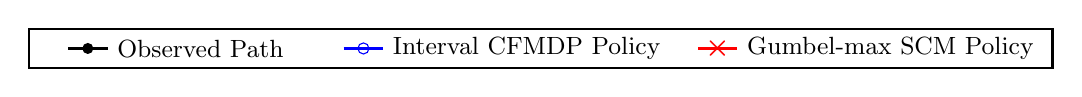
\begin{tikzpicture}[scale=1.0, every node/.style={scale=1.0}]
            \draw[thick, black] (-3, -0.25) rectangle (10, 0.25);
            %
            \draw[black, line width=1pt] (-2.5, 0.0) -- (-2,0.0);
            \fill[black] (-2.25,0.0) circle (2pt); %
            \node[right] at (-2,0.0) {\small Observed Path};
            
            %
            \draw[blue, line width=1pt] (1.0,0.0) -- (1.5,0.0);
            \node[draw=blue, circle, minimum size=4pt, inner sep=0pt] at (1.25,0.0) {}; %
            \node[right] at (1.5,0.0) {\small Interval CFMDP Policy};
            
            %
            \draw[red, line width=1pt] (5.5,0) -- (6,0);
            \node[red] at (5.75,0) {$\boldsymbol{\times}$}; %
            \node[right] at (6,0) {\small Gumbel-max SCM Policy};
        \end{tikzpicture}
    }\\
    %
    \subfigure[\footnotesize Lowest cumulative reward: Interval CFMDP ($312$), Gumbel-max SCM ($312$)]{%
        \resizebox{0.76\columnwidth}{!}{
             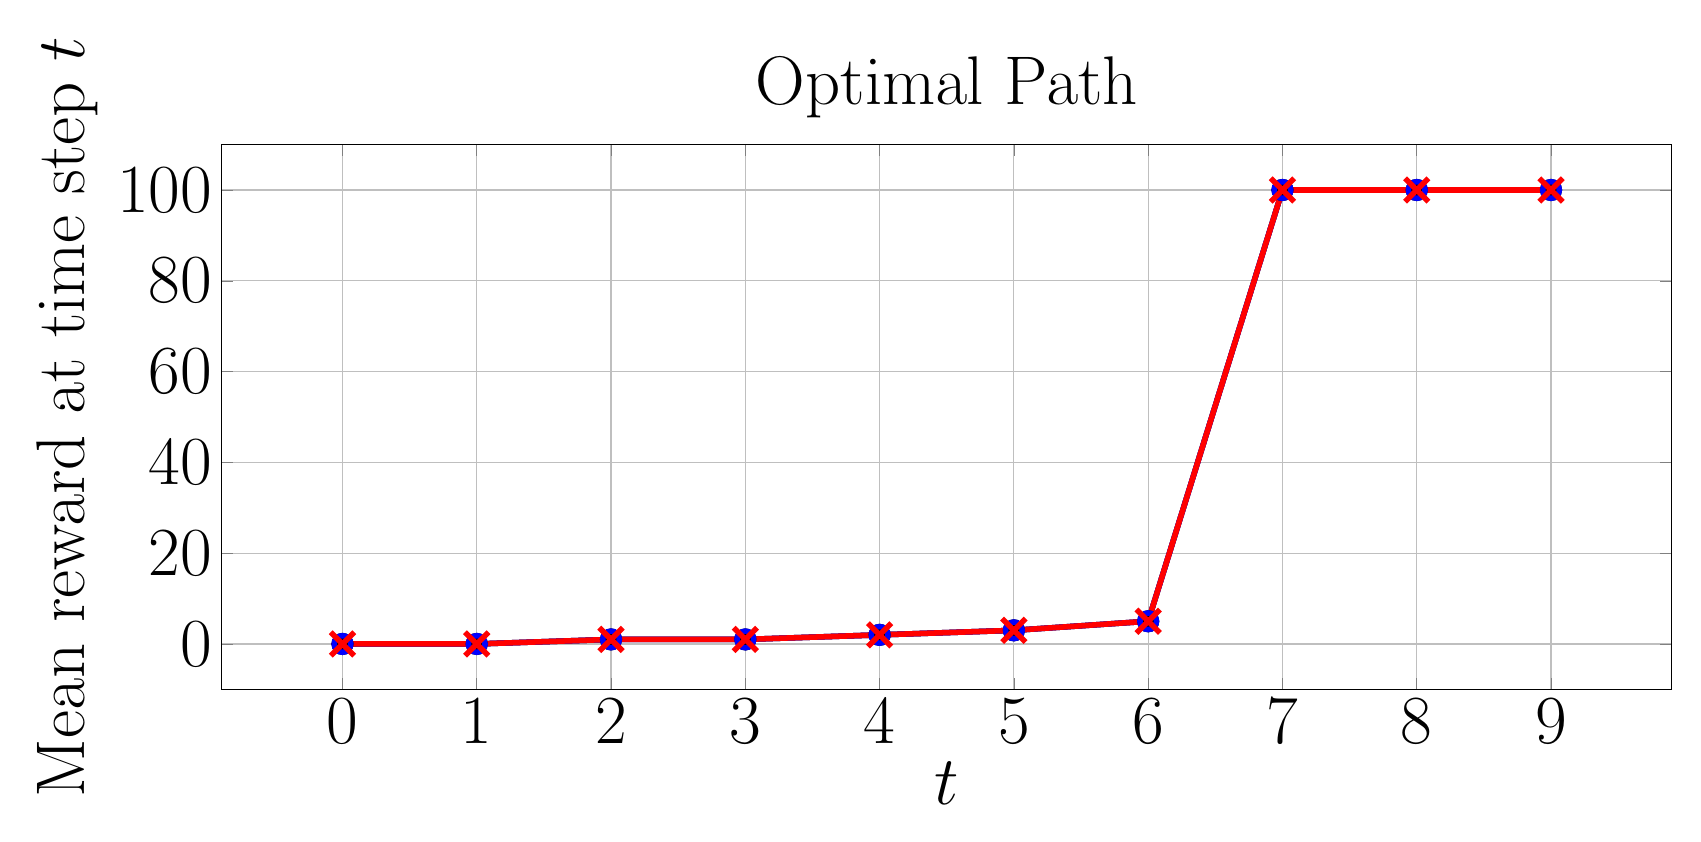
\begin{tikzpicture}
                \begin{axis}[
                    xlabel={$t$},
                    ylabel={Mean reward at time step $t$},
                    title={Optimal Path},
                    grid=both,
                    width=20cm, height=8.5cm,
                    every axis/.style={font=\Huge},
                    %
                ]
                \addplot[
                    color=black, %
                    mark=*, %
                    line width=2pt,
                    mark size=3pt,
                    error bars/.cd,
                    y dir=both, %
                    y explicit, %
                    error bar style={line width=1pt,solid},
                    error mark options={line width=1pt,mark size=4pt,rotate=90}
                ]
                coordinates {
                    (0, 0.0)  +- (0, 0.0)
                    (1, 0.0)  +- (0, 0.0) 
                    (2, 1.0)  +- (0, 0.0) 
                    (3, 1.0)  +- (0, 0.0)
                    (4, 2.0)  +- (0, 0.0)
                    (5, 3.0) +- (0, 0.0)
                    (6, 5.0) +- (0, 0.0)
                    (7, 100.0) +- (0, 0.0)
                    (8, 100.0) +- (0, 0.0)
                    (9, 100.0) +- (0, 0.0)
                };
                %
                \addplot[
                    color=blue, %
                    mark=o, %
                    line width=2pt,
                    mark size=3pt,
                    error bars/.cd,
                    y dir=both, %
                    y explicit, %
                    error bar style={line width=1pt,solid},
                    error mark options={line width=1pt,mark size=4pt,rotate=90}
                ]
                 coordinates {
                    (0, 0.0)  +- (0, 0.0)
                    (1, 0.0)  +- (0, 0.0) 
                    (2, 1.0)  +- (0, 0.0) 
                    (3, 1.0)  +- (0, 0.0)
                    (4, 2.0)  +- (0, 0.0)
                    (5, 3.0) +- (0, 0.0)
                    (6, 5.0) +- (0, 0.0)
                    (7, 100.0) +- (0, 0.0)
                    (8, 100.0) +- (0, 0.0)
                    (9, 100.0) +- (0, 0.0)
                };
                %
                \addplot[
                    color=red, %
                    mark=x, %
                    line width=2pt,
                    mark size=6pt,
                    error bars/.cd,
                    y dir=both, %
                    y explicit, %
                    error bar style={line width=1pt,solid},
                    error mark options={line width=1pt,mark size=4pt,rotate=90}
                ]
                coordinates {
                    (0, 0.0)  +- (0, 0.0)
                    (1, 0.0)  +- (0, 0.0) 
                    (2, 1.0)  +- (0, 0.0) 
                    (3, 1.0)  +- (0, 0.0)
                    (4, 2.0)  +- (0, 0.0)
                    (5, 3.0) +- (0, 0.0)
                    (6, 5.0) +- (0, 0.0)
                    (7, 100.0) +- (0, 0.0)
                    (8, 100.0) +- (0, 0.0)
                    (9, 100.0) +- (0, 0.0)
                };
                \end{axis}
            \end{tikzpicture}
         }
    }
    \hspace{1cm}
    \subfigure[\footnotesize Lowest cumulative reward: Interval CFMDP ($19$), Gumbel-max SCM ($-88$)]{%
         \resizebox{0.76\columnwidth}{!}{
            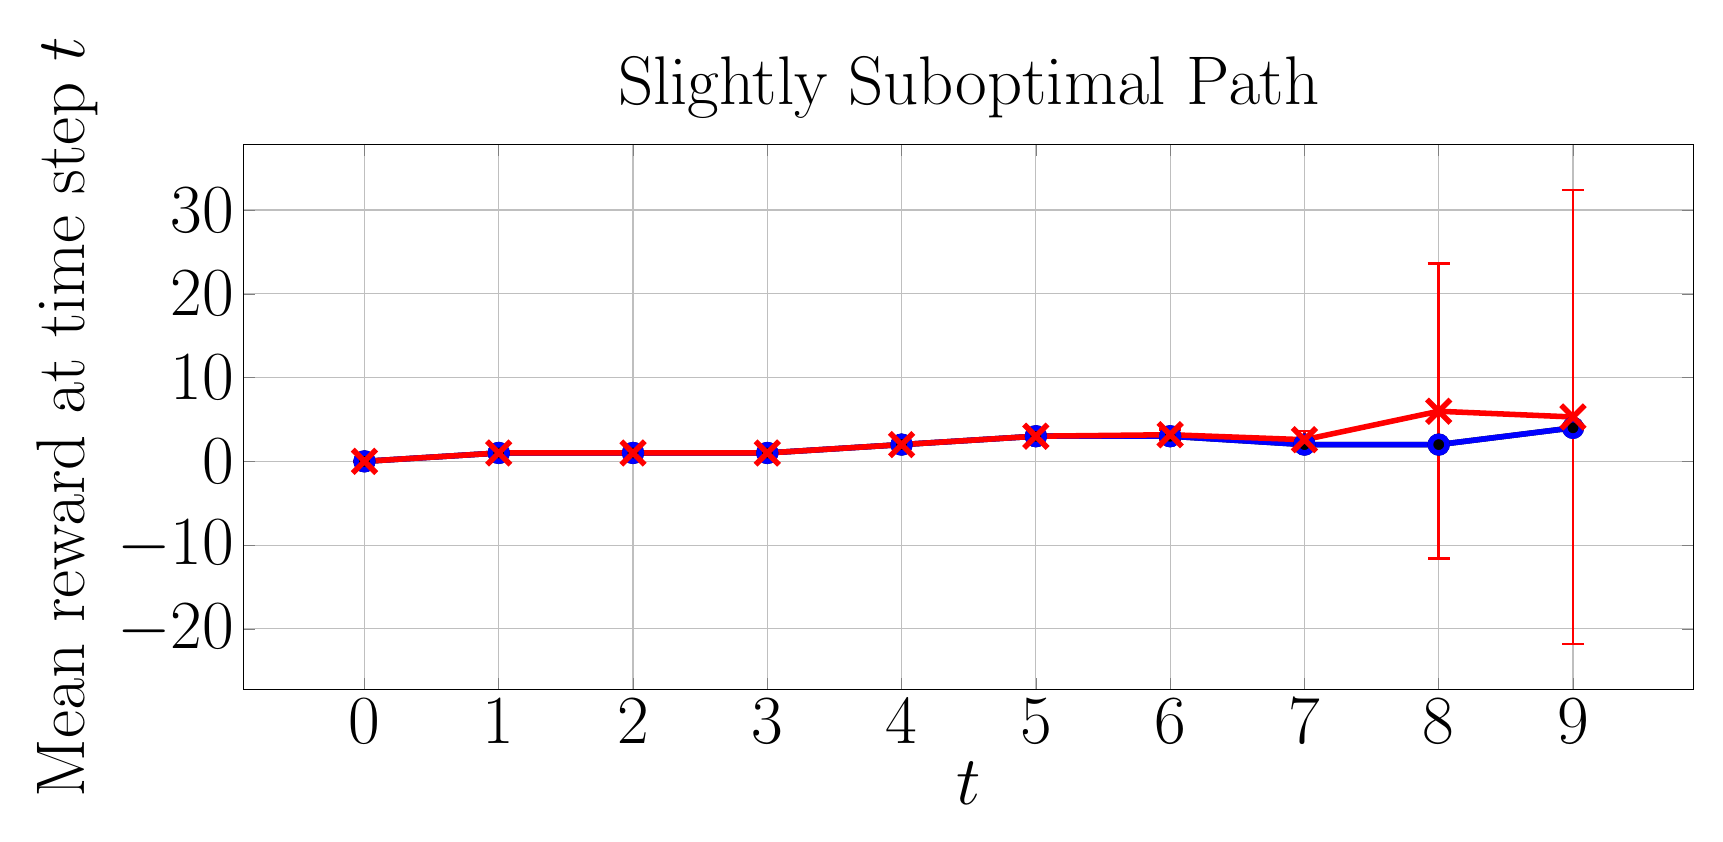
\begin{tikzpicture}
                \begin{axis}[
                    xlabel={$t$},
                    ylabel={Mean reward at time step $t$},
                    title={Slightly Suboptimal Path},
                    grid=both,
                    width=20cm, height=8.5cm,
                    every axis/.style={font=\Huge},
                    %
                ]
                \addplot[
                    color=black, %
                    mark=*, %
                    line width=2pt,
                    mark size=3pt,
                    error bars/.cd,
                    y dir=both, %
                    y explicit, %
                    error bar style={line width=1pt,solid},
                    error mark options={line width=1pt,mark size=4pt,rotate=90}
                ]
              coordinates {
                    (0, 0.0)  +- (0, 0.0)
                    (1, 1.0)  +- (0, 0.0) 
                    (2, 1.0)  +- (0, 0.0) 
                    (3, 1.0)  +- (0, 0.0)
                    (4, 2.0)  +- (0, 0.0)
                    (5, 3.0) +- (0, 0.0)
                    (6, 3.0) +- (0, 0.0)
                    (7, 2.0) +- (0, 0.0)
                    (8, 2.0) +- (0, 0.0)
                    (9, 4.0) +- (0, 0.0)
                };
                %
                \addplot[
                    color=blue, %
                    mark=o, %
                    line width=2pt,
                    mark size=3pt,
                    error bars/.cd,
                    y dir=both, %
                    y explicit, %
                    error bar style={line width=1pt,solid},
                    error mark options={line width=1pt,mark size=4pt,rotate=90}
                ]
              coordinates {
                    (0, 0.0)  +- (0, 0.0)
                    (1, 1.0)  +- (0, 0.0) 
                    (2, 1.0)  +- (0, 0.0) 
                    (3, 1.0)  +- (0, 0.0)
                    (4, 2.0)  +- (0, 0.0)
                    (5, 3.0) +- (0, 0.0)
                    (6, 3.0) +- (0, 0.0)
                    (7, 2.0) +- (0, 0.0)
                    (8, 2.0) +- (0, 0.0)
                    (9, 4.0) +- (0, 0.0)
                };
                %
                \addplot[
                    color=red, %
                    mark=x, %
                    line width=2pt,
                    mark size=6pt,
                    error bars/.cd,
                    y dir=both, %
                    y explicit, %
                    error bar style={line width=1pt,solid},
                    error mark options={line width=1pt,mark size=4pt,rotate=90}
                ]
                coordinates {
                    (0, 0.0)  +- (0, 0.0)
                    (1, 1.0)  +- (0, 0.0) 
                    (2, 1.0)  +- (0, 0.0) 
                    (3, 1.0)  +- (0, 0.0)
                    (4, 2.0)  += (0, 0.0)
                    (5, 3.0)  += (0, 0.0)
                    (6, 3.17847) += (0, 0.62606746) -= (0, 0.62606746)
                    (7, 2.5832885) += (0, 1.04598233) -= (0, 1.04598233)
                    (8, 5.978909) += (0, 17.60137623) -= (0, 17.60137623)
                    (9, 5.297059) += (0, 27.09227512) -= (0, 27.09227512)
                };
                \end{axis}
            \end{tikzpicture}
         }
    }\\[-1.5pt]
    \subfigure[\footnotesize Lowest cumulative reward: Interval CFMDP ($14$), Gumbel-max SCM ($-598$)]{%
         \resizebox{0.76\columnwidth}{!}{
             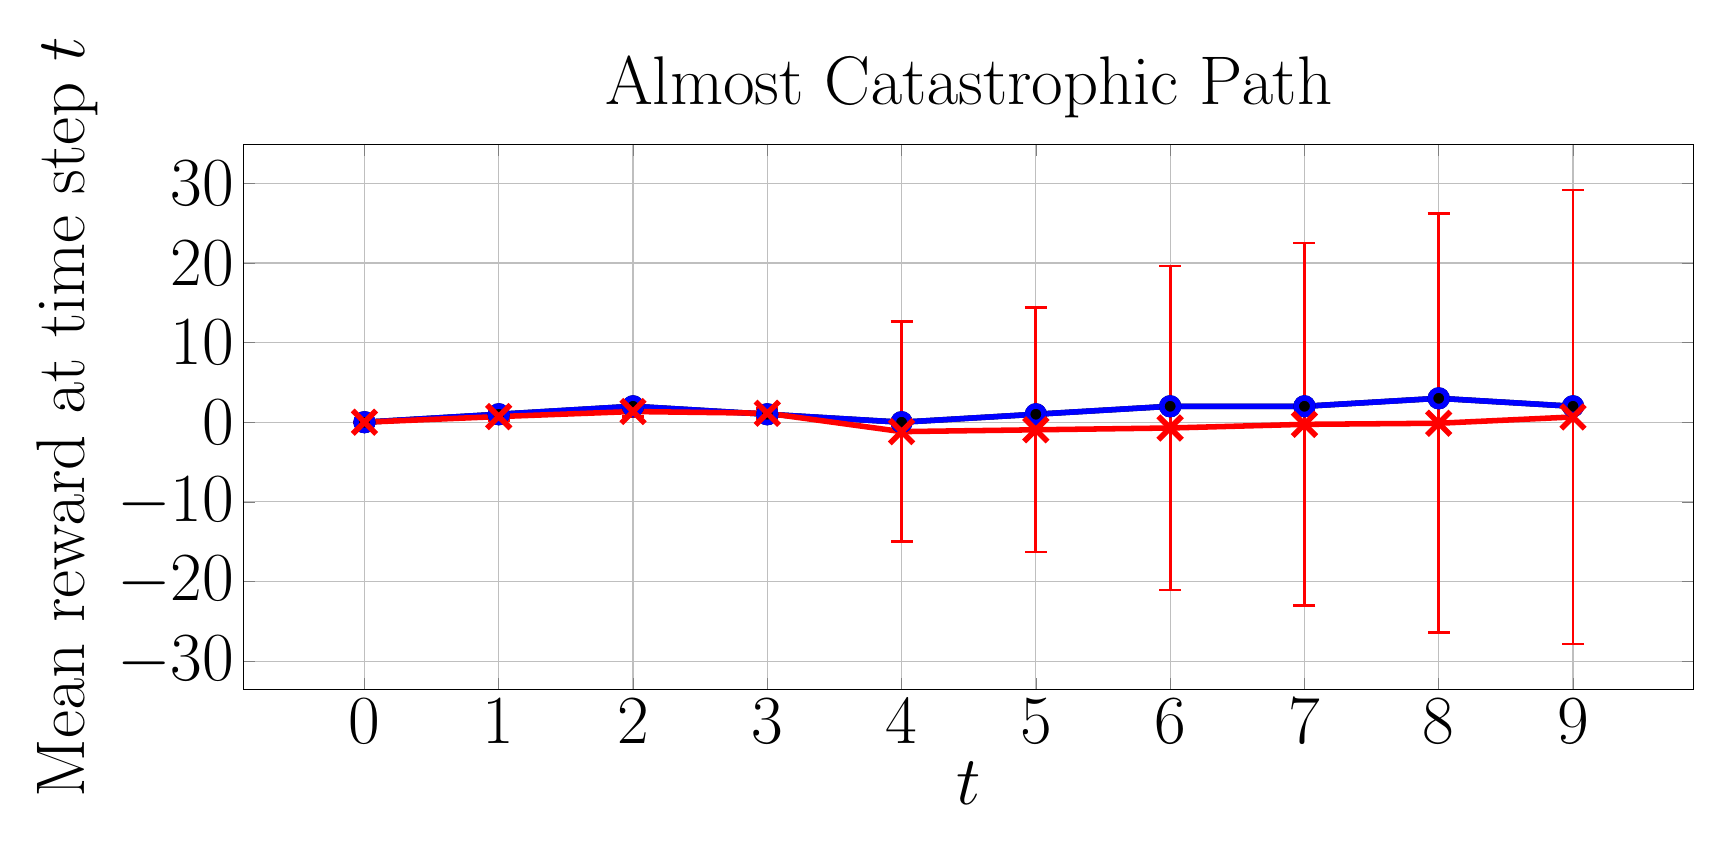
\begin{tikzpicture}
                \begin{axis}[
                    xlabel={$t$},
                    ylabel={Mean reward at time step $t$},
                    title={Almost Catastrophic Path},
                    grid=both,
                    width=20cm, height=8.5cm,
                    every axis/.style={font=\Huge},
                    %
                ]
                \addplot[
                    color=black, %
                    mark=*, %
                    line width=2pt,
                    mark size=3pt,
                    error bars/.cd,
                    y dir=both, %
                    y explicit, %
                    error bar style={line width=1pt,solid},
                    error mark options={line width=1pt,mark size=4pt,rotate=90}
                ]
                coordinates {
                    (0, 0.0)  +- (0, 0.0)
                    (1, 1.0)  +- (0, 0.0) 
                    (2, 2.0)  +- (0, 0.0) 
                    (3, 1.0)  +- (0, 0.0)
                    (4, 0.0)  +- (0, 0.0)
                    (5, 1.0) +- (0, 0.0)
                    (6, 2.0) +- (0, 0.0)
                    (7, 2.0) +- (0, 0.0)
                    (8, 3.0) +- (0, 0.0)
                    (9, 2.0) +- (0, 0.0)
                };
                %
                \addplot[
                    color=blue, %
                    mark=o, %
                    line width=2pt,
                    mark size=3pt,
                    error bars/.cd,
                    y dir=both, %
                    y explicit, %
                    error bar style={line width=1pt,solid},
                    error mark options={line width=1pt,mark size=4pt,rotate=90}
                ]
                coordinates {
                    (0, 0.0)  +- (0, 0.0)
                    (1, 1.0)  +- (0, 0.0) 
                    (2, 2.0)  +- (0, 0.0) 
                    (3, 1.0)  +- (0, 0.0)
                    (4, 0.0)  +- (0, 0.0)
                    (5, 1.0) +- (0, 0.0)
                    (6, 2.0) +- (0, 0.0)
                    (7, 2.0) +- (0, 0.0)
                    (8, 3.0) +- (0, 0.0)
                    (9, 2.0) +- (0, 0.0)
                };
                %
                \addplot[
                    color=red, %
                    mark=x, %
                    line width=2pt,
                    mark size=6pt,
                    error bars/.cd,
                    y dir=both, %
                    y explicit, %
                    error bar style={line width=1pt,solid},
                    error mark options={line width=1pt,mark size=4pt,rotate=90}
                ]
                coordinates {
                    (0, 0.0)  +- (0, 0.0)
                    (1, 0.7065655)  +- (0, 0.4553358) 
                    (2, 1.341673)  +- (0, 0.67091621) 
                    (3, 1.122926)  +- (0, 0.61281824)
                    (4, -1.1821935)  +- (0, 13.82444042)
                    (5, -0.952399)  +- (0, 15.35195457)
                    (6, -0.72672) +- (0, 20.33508414)
                    (7, -0.268983) +- (0, 22.77861454)
                    (8, -0.1310835) +- (0, 26.31013314)
                    (9, 0.65806) +- (0, 28.50670214)
                };
                %
            %
            %
            %
            %
            %
            %
            %
            %
            %
            %
            %
            %
            %
            %
            %
            %
            %
            %
                \end{axis}
            \end{tikzpicture}
         }
    }
    \hspace{1cm}
    \subfigure[\footnotesize Lowest cumulative reward: Interval CFMDP ($-698$), Gumbel-max SCM ($-698$)]{%
         \resizebox{0.76\columnwidth}{!}{
            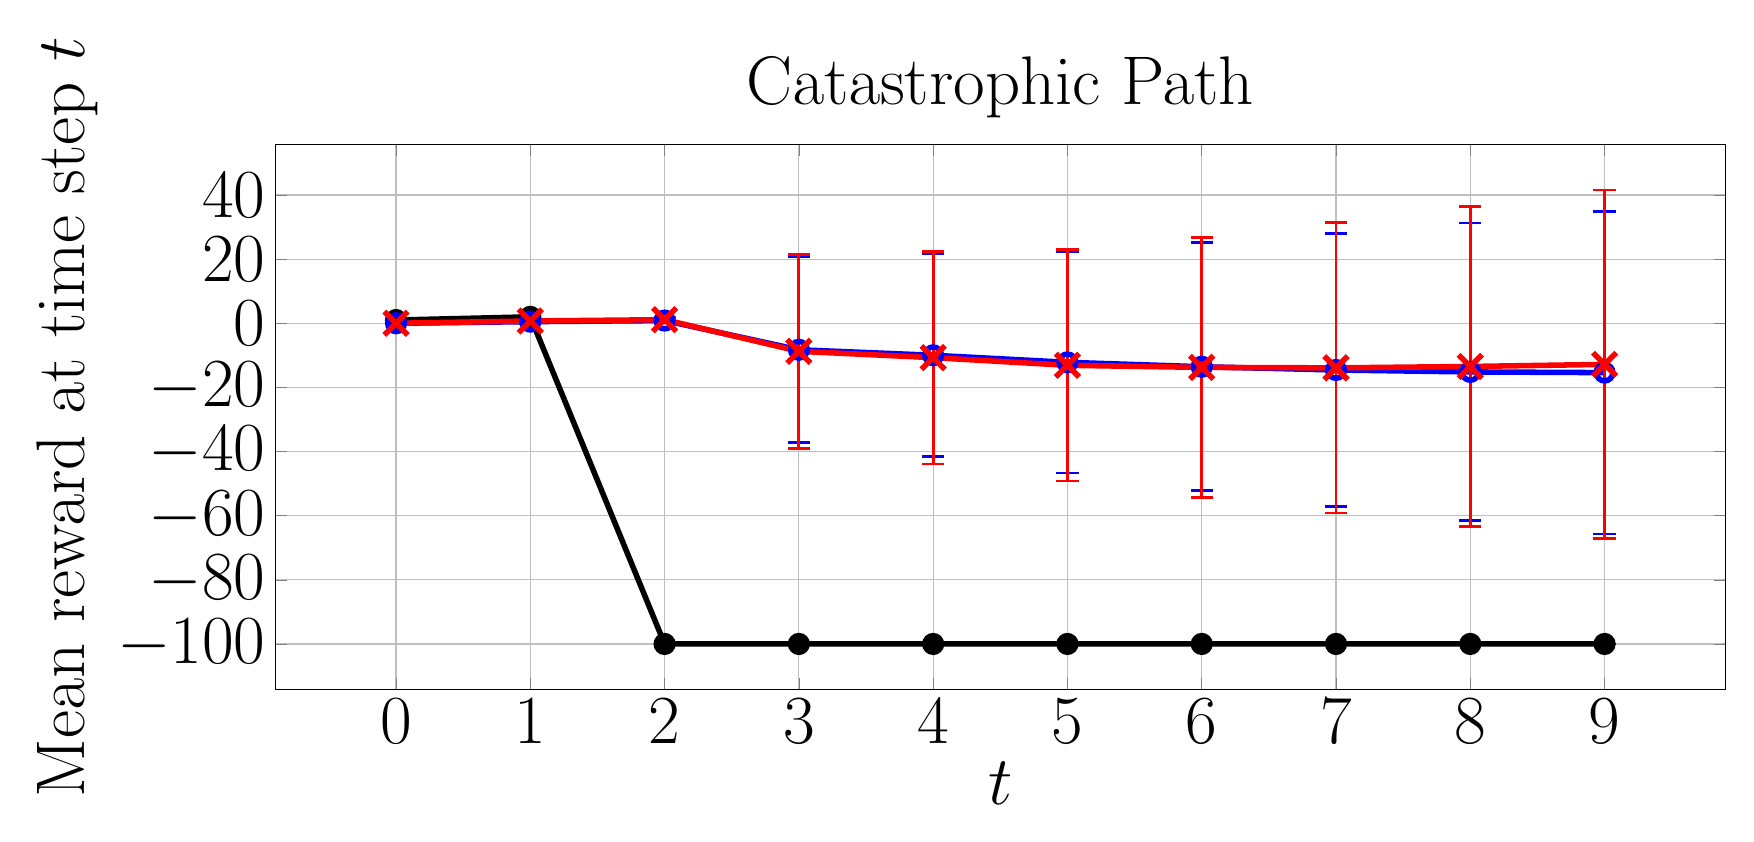
\begin{tikzpicture}
                \begin{axis}[
                    xlabel={$t$},
                    ylabel={Mean reward at time step $t$},
                    title={Catastrophic Path},
                    grid=both,
                    width=20cm, height=8.5cm,
                    every axis/.style={font=\Huge},
                    %
                ]
                \addplot[
                    color=black, %
                    mark=*, %
                    line width=2pt,
                    mark size=3pt,
                    error bars/.cd,
                    y dir=both, %
                    y explicit, %
                    error bar style={line width=1pt,solid},
                    error mark options={line width=1pt,mark size=4pt,rotate=90}
                ]
                coordinates {
                    (0, 1.0)  +- (0, 0.0)
                    (1, 2.0)  +- (0, 0.0) 
                    (2, -100.0)  +- (0, 0.0) 
                    (3, -100.0)  +- (0, 0.0)
                    (4, -100.0)  +- (0, 0.0)
                    (5, -100.0) +- (0, 0.0)
                    (6, -100.0) +- (0, 0.0)
                    (7, -100.0) +- (0, 0.0)
                    (8, -100.0) +- (0, 0.0)
                    (9, -100.0) +- (0, 0.0)
                };
                %
                \addplot[
                    color=blue, %
                    mark=o, %
                    line width=2pt,
                    mark size=3pt,
                    error bars/.cd,
                    y dir=both, %
                    y explicit, %
                    error bar style={line width=1pt,solid},
                    error mark options={line width=1pt,mark size=4pt,rotate=90}
                ]
                coordinates {
                    (0, 0.0)  +- (0, 0.0)
                    (1, 0.504814)  +- (0, 0.49997682) 
                    (2, 0.8439835)  +- (0, 0.76831917) 
                    (3, -8.2709165)  +- (0, 28.93656754)
                    (4, -9.981082)  +- (0, 31.66825363)
                    (5, -12.1776325) +- (0, 34.53463233)
                    (6, -13.556076) +- (0, 38.62845372)
                    (7, -14.574418) +- (0, 42.49603359)
                    (8, -15.1757075) +- (0, 46.41913968)
                    (9, -15.3900395) +- (0, 50.33563368)
                };
                %
                \addplot[
                    color=red, %
                    mark=x, %
                    line width=2pt,
                    mark size=6pt,
                    error bars/.cd,
                    y dir=both, %
                    y explicit, %
                    error bar style={line width=1pt,solid},
                    error mark options={line width=1pt,mark size=4pt,rotate=90}
                ]
                coordinates {
                    (0, 0.0)  +- (0, 0.0)
                    (1, 0.701873)  +- (0, 0.45743556) 
                    (2, 1.1227805)  +- (0, 0.73433129) 
                    (3, -8.7503255)  +- (0, 30.30257976)
                    (4, -10.722092)  +- (0, 33.17618589)
                    (5, -13.10721)  +- (0, 36.0648089)
                    (6, -13.7631645) +- (0, 40.56553451)
                    (7, -13.909043) +- (0, 45.23829402)
                    (8, -13.472517) +- (0, 49.96270296)
                    (9, -12.8278835) +- (0, 54.38618735)
                };
                %
            %
            %
            %
            %
            %
            %
            %
            %
            %
            %
            %
            %
            %
            %
            %
            %
            %
            %
                \end{axis}
            \end{tikzpicture}
         }
    }
    \caption{Average instant reward of CF paths induced by policies on GridWorld $p=0.4$.}
    \label{fig: reward p=0.4}
\end{figure*}

\subsection{Experimental Setup}
To compare policy performance, we measure the average rewards of counterfactual paths induced by our policy and the Gumbel-max policy by uniformly sampling $200$ counterfactual MDPs from the ICFMDP and generating $10,000$ counterfactual paths over each sampled CFMDP. \jl{Since the interval CFMDP depends on the observed path, we select $4$  paths of varying optimality to evaluate how the observed path impacts the performance of both policies: an optimal path, a slightly suboptimal path that could reach the optimal reward with a few changes, a catastrophic path that enters a catastrophic, terminal state with low reward, and an almost catastrophic path that was close to entering a catastrophic state.} When measuring the average probability bound widths and execution time needed to generate the ICFMDPs, we averaged over $20$ randomly generated observed paths
\footnote{Further training details are provided in Appendix \ref{app: training details}, and the code is provided at \href{https://github.com/ddv-lab/robust-cf-inference-in-MDPs}{https://github.com/ddv-lab/robust-cf-inference-in-MDPs}
%
%
.}.

\subsection{GridWorld}
\jl{The GridWorld MDP is a $4 \times 4$ grid where an agent must navigate from the top-left corner to the goal state in the bottom-right corner, avoiding a dangerous terminal state in the centre. At each time step, the agent can move up, down, left, or right, but there is a small probability (controlled by hyper-parameter $p$) of moving in an unintended direction. As the agent nears the goal, the reward for each state increases, culminating in a reward of $+100$ for reaching the goal. Entering the dangerous state results in a penalty of $-100$. We use two versions of GridWorld: a less stochastic version with $p=0.9$ (i.e., $90$\% chance of moving in the chosen direction) and a more stochastic version with $p=0.4$.}

\paragraph{GridWorld ($p=0.9$)}
When $p=0.9$, the counterfactual probability bounds are typically narrow (see Table \ref{tab:nonzero_probs} for average measurements). Consequently, as shown in Figure \ref{fig: reward p=0.9}, both policies are nearly identical and perform similarly well across the optimal, slightly suboptimal, and catastrophic paths.
%
However, for the almost catastrophic path, the interval CFMDP path is more conservative and follows the observed path more closely (as this is where the probability bounds are narrowest), which typically requires one additional step to reach the goal state than the Gumbel-max SCM policy.
%

\paragraph{GridWorld ($p=0.4$)}
\jl{When $p=0.4$, the GridWorld environment becomes more uncertain, increasing the risk of entering the dangerous state even if correct actions are chosen. Thus, as shown in Figure \ref{fig: reward p=0.4}, the interval CFMDP policy adopts a more conservative approach, avoiding deviation from the observed policy if it cannot guarantee higher counterfactual rewards (see the slightly suboptimal and almost catastrophic paths), whereas the Gumbel-max SCM is inconsistent: it can yield higher rewards, but also much lower rewards, reflected in the wide error bars.} For the catastrophic path, both policies must deviate from the observed path to achieve a higher reward and, in this case, perform similarly.
%
%
%
%
\subsection{Sepsis}
The Sepsis MDP \citep{oberst2019counterfactual} simulates trajectories of Sepsis patients. Each state consists of four vital signs (heart rate, blood pressure, oxygen concentration, and glucose levels), categorised as low, normal, or high.
and three treatments that can be toggled on/off at each time step (8 actions in total). Unlike \citet{oberst2019counterfactual}, we scale rewards based on the number of out-of-range vital signs, between $-1000$ (patient dies) and $1000$ (patient discharged). \jl{Like the GridWorld $p=0.4$ experiment, the Sepsis MDP is highly uncertain, as many states are equally likely to lead to optimal and poor outcomes. Thus, as shown in Figure \ref{fig: reward sepsis}, both policies follow the observed optimal and almost catastrophic paths to guarantee rewards are no worse than the observation.} However, improving the catastrophic path requires deviating from the observation. Here, the Gumbel-max SCM policy, on average, performs better than the interval CFMDP policy. But, since both policies have lower bounds clipped at $-1000$, neither policy reliably improves over the observation. In contrast, for the slightly suboptimal path, the interval CFMDP policy performs significantly better, shown by its higher lower bounds. 
Moreover, in these two cases, the worst-case counterfactual path generated by the interval CFMDP policy is better than that of the Gumbel-max SCM policy,
indicating its greater robustness.
%
\begin{figure*}
    \centering
     \resizebox{0.6\textwidth}{!}{
        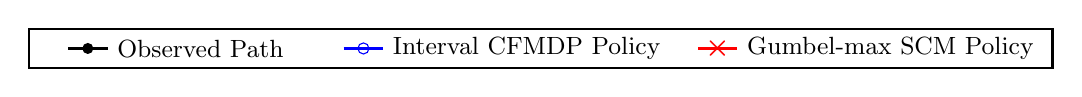
\begin{tikzpicture}[scale=1.0, every node/.style={scale=1.0}]
            \draw[thick, black] (-3, -0.25) rectangle (10, 0.25);
            %
            \draw[black, line width=1pt] (-2.5, 0.0) -- (-2,0.0);
            \fill[black] (-2.25,0.0) circle (2pt); %
            \node[right] at (-2,0.0) {\small Observed Path};
            
            %
            \draw[blue, line width=1pt] (1.0,0.0) -- (1.5,0.0);
            \node[draw=blue, circle, minimum size=4pt, inner sep=0pt] at (1.25,0.0) {}; %
            \node[right] at (1.5,0.0) {\small Interval CFMDP Policy};
            
            %
            \draw[red, line width=1pt] (5.5,0) -- (6,0);
            \node[red] at (5.75,0) {$\boldsymbol{\times}$}; %
            \node[right] at (6,0) {\small Gumbel-max SCM Policy};
        \end{tikzpicture}
    }\\
    \subfigure[\footnotesize Lowest cumulative reward: Interval CFMDP ($8000$), Gumbel-max SCM ($8000$)]{%
         \resizebox{0.76\columnwidth}{!}{
             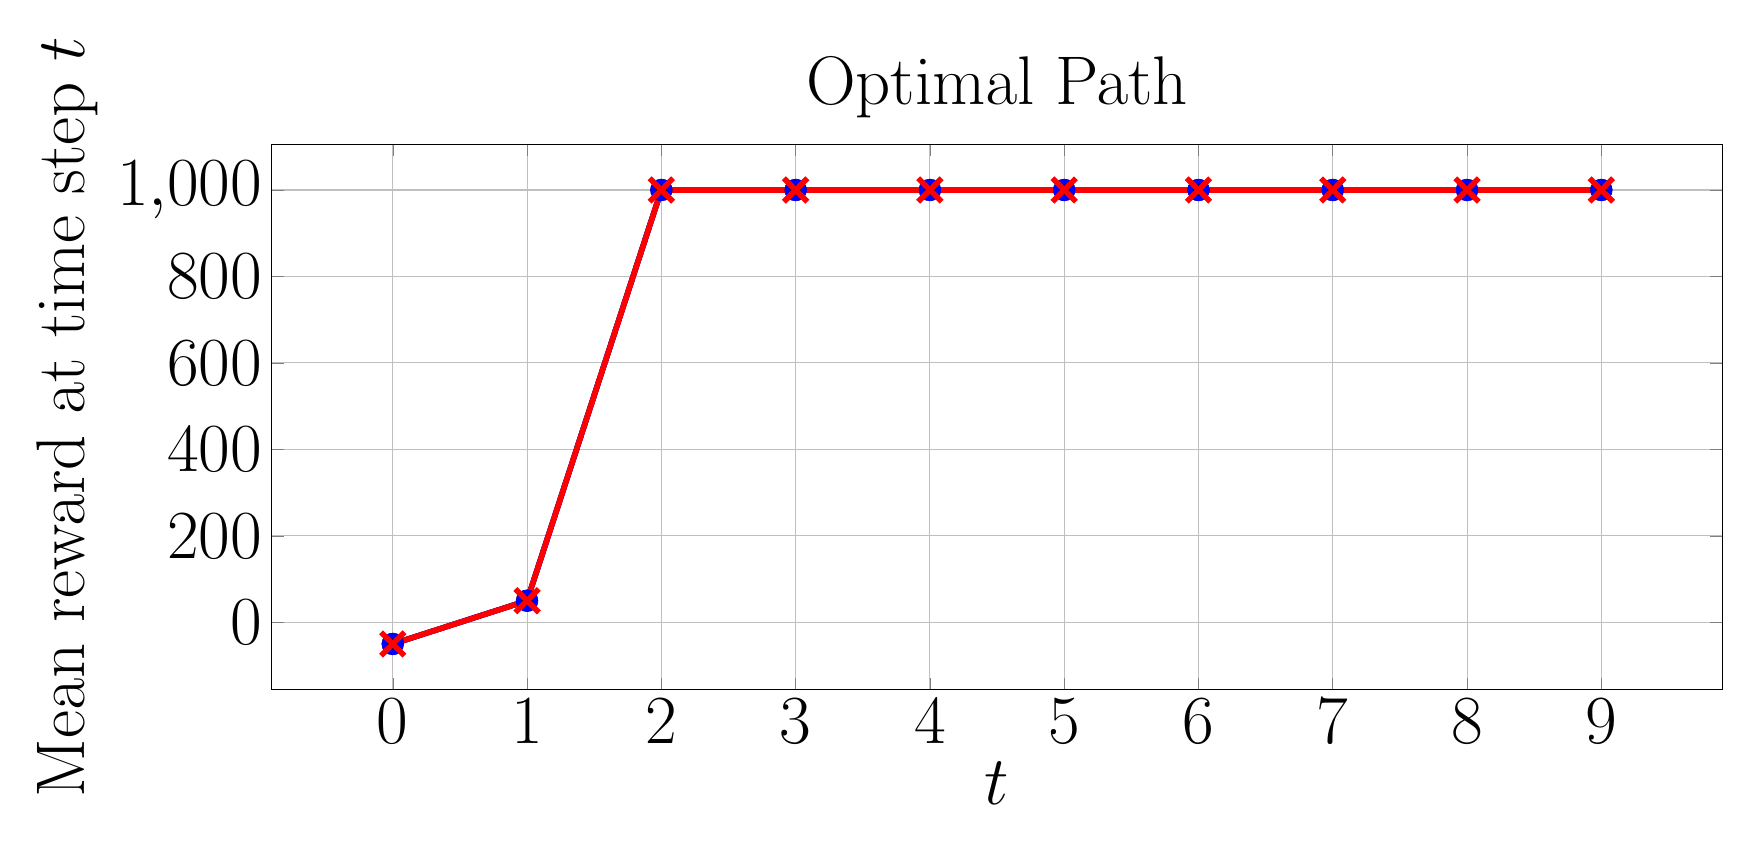
\begin{tikzpicture}
                \begin{axis}[
                    xlabel={$t$},
                    ylabel={Mean reward at time step $t$},
                    title={Optimal Path},
                    grid=both,
                    width=20cm, height=8.5cm,
                    every axis/.style={font=\Huge},
                    %
                ]
                \addplot[
                    color=black, %
                    mark=*, %
                    line width=2pt,
                    mark size=3pt,
                ]
                coordinates {
                    (0, -50.0)
                    (1, 50.0)
                    (2, 1000.0)
                    (3, 1000.0)
                    (4, 1000.0)
                    (5, 1000.0)
                    (6, 1000.0)
                    (7, 1000.0)
                    (8, 1000.0)
                    (9, 1000.0)
                };
                %
                \addplot[
                    color=blue, %
                    mark=o, %
                    line width=2pt,
                    mark size=3pt,
                    error bars/.cd,
                    y dir=both, %
                    y explicit, %
                    error bar style={line width=1pt,solid},
                    error mark options={line width=1pt,mark size=4pt,rotate=90}
                ]
                coordinates {
                    (0, -50.0)  +- (0, 0.0)
                    (1, 50.0)  +- (0, 0.0) 
                    (2, 1000.0)  +- (0, 0.0) 
                    (3, 1000.0)  +- (0, 0.0)
                    (4, 1000.0)  +- (0, 0.0)
                    (5, 1000.0) +- (0, 0.0)
                    (6, 1000.0) +- (0, 0.0)
                    (7, 1000.0) +- (0, 0.0)
                    (8, 1000.0) +- (0, 0.0)
                    (9, 1000.0) +- (0, 0.0)
                };
                %
                \addplot[
                    color=red, %
                    mark=x, %
                    line width=2pt,
                    mark size=6pt,
                    error bars/.cd,
                    y dir=both, %
                    y explicit, %
                    error bar style={line width=1pt,solid},
                    error mark options={line width=1pt,mark size=4pt,rotate=90}
                ]
                coordinates {
                    (0, -50.0)  +- (0, 0.0)
                    (1, 50.0)  +- (0, 0.0) 
                    (2, 1000.0)  +- (0, 0.0) 
                    (3, 1000.0)  +- (0, 0.0)
                    (4, 1000.0)  +- (0, 0.0)
                    (5, 1000.0) +- (0, 0.0)
                    (6, 1000.0) +- (0, 0.0)
                    (7, 1000.0) +- (0, 0.0)
                    (8, 1000.0) +- (0, 0.0)
                    (9, 1000.0) +- (0, 0.0)
                };
                %
                \end{axis}
            \end{tikzpicture}
         }
    }
    \hspace{1cm}
    \subfigure[\footnotesize Lowest cumulative reward: Interval CFMDP ($-5980$), Gumbel-max SCM ($-8000$)]{%
         \resizebox{0.76\columnwidth}{!}{
            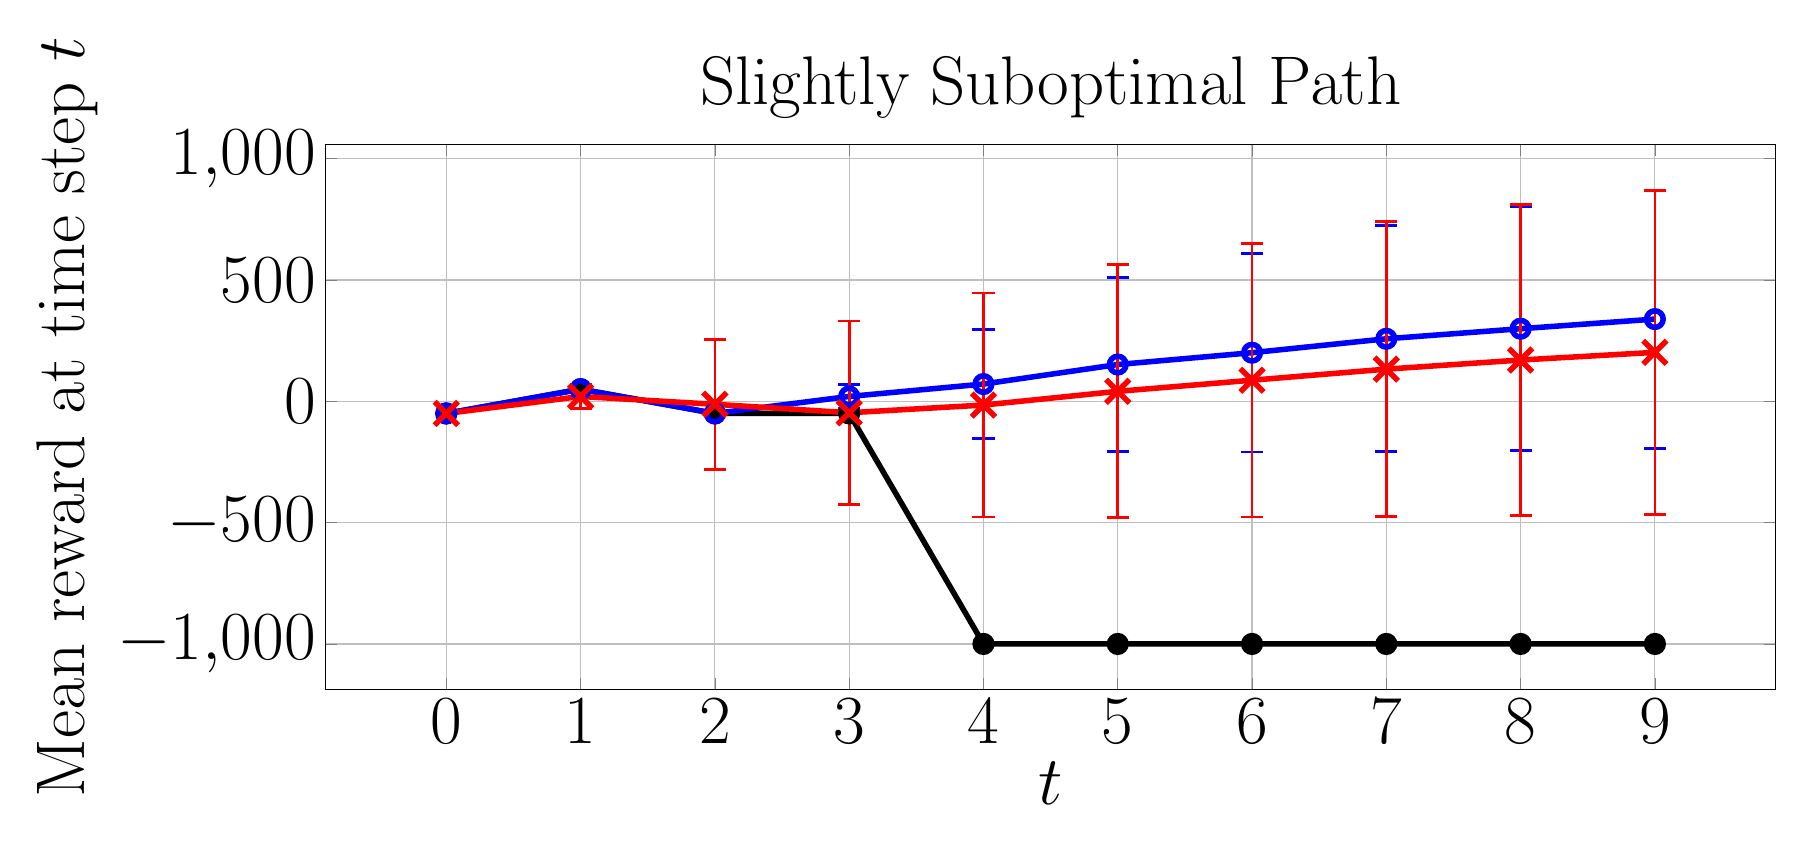
\begin{tikzpicture}
                \begin{axis}[
                    xlabel={$t$},
                    ylabel={Mean reward at time step $t$},
                    title={Slightly Suboptimal Path},
                    grid=both,
                    width=20cm, height=8.5cm,
                    every axis/.style={font=\Huge},
                    %
                ]
               \addplot[
                    color=black, %
                    mark=*, %
                    line width=2pt,
                    mark size=3pt,
                ]
                coordinates {
                    (0, -50.0)
                    (1, 50.0)
                    (2, -50.0)
                    (3, -50.0)
                    (4, -1000.0)
                    (5, -1000.0)
                    (6, -1000.0)
                    (7, -1000.0)
                    (8, -1000.0)
                    (9, -1000.0)
                };
                %
                \addplot[
                    color=blue, %
                    mark=o, %
                    line width=2pt,
                    mark size=3pt,
                    error bars/.cd,
                    y dir=both, %
                    y explicit, %
                    error bar style={line width=1pt,solid},
                    error mark options={line width=1pt,mark size=4pt,rotate=90}
                ]
                coordinates {
                    (0, -50.0)  +- (0, 0.0)
                    (1, 50.0)  +- (0, 0.0) 
                    (2, -50.0)  +- (0, 0.0) 
                    (3, 20.0631)  +- (0, 49.97539413)
                    (4, 71.206585)  +- (0, 226.02033693)
                    (5, 151.60797) +- (0, 359.23292559)
                    (6, 200.40593) +- (0, 408.86185176)
                    (7, 257.77948) +- (0, 466.10372804)
                    (8, 299.237465) +- (0, 501.82579506)
                    (9, 338.9129) +- (0, 532.06124996)
                };
                %
                \addplot[
                    color=red, %
                    mark=x, %
                    line width=2pt,
                    mark size=6pt,
                    error bars/.cd,
                    y dir=both, %
                    y explicit, %
                    error bar style={line width=1pt,solid},
                    error mark options={line width=1pt,mark size=4pt,rotate=90}
                ]
                coordinates {
                    (0, -50.0)  +- (0, 0.0)
                    (1, 20.00736)  +- (0, 49.99786741) 
                    (2, -12.282865)  +- (0, 267.598755) 
                    (3, -47.125995)  +- (0, 378.41755832)
                    (4, -15.381965)  +- (0, 461.77616558)
                    (5, 41.15459) +- (0, 521.53189262)
                    (6, 87.01595) +- (0, 564.22243126 )
                    (7, 132.62376) +- (0, 607.31338037)
                    (8, 170.168145) +- (0, 641.48013693)
                    (9, 201.813135) +- (0, 667.29441777)
                };
                %
                %
                %
                %
                %
                %
                %
                %
                %
                %
                %
                %
                %
                %
                %
                %
                %
                %
                %
                \end{axis}
            \end{tikzpicture}
         }
    }\\[-1.5pt]
    \subfigure[\footnotesize Lowest cumulative reward: Interval CFMDP ($100$), Gumbel-max SCM ($100$)]{%
         \resizebox{0.76\columnwidth}{!}{
             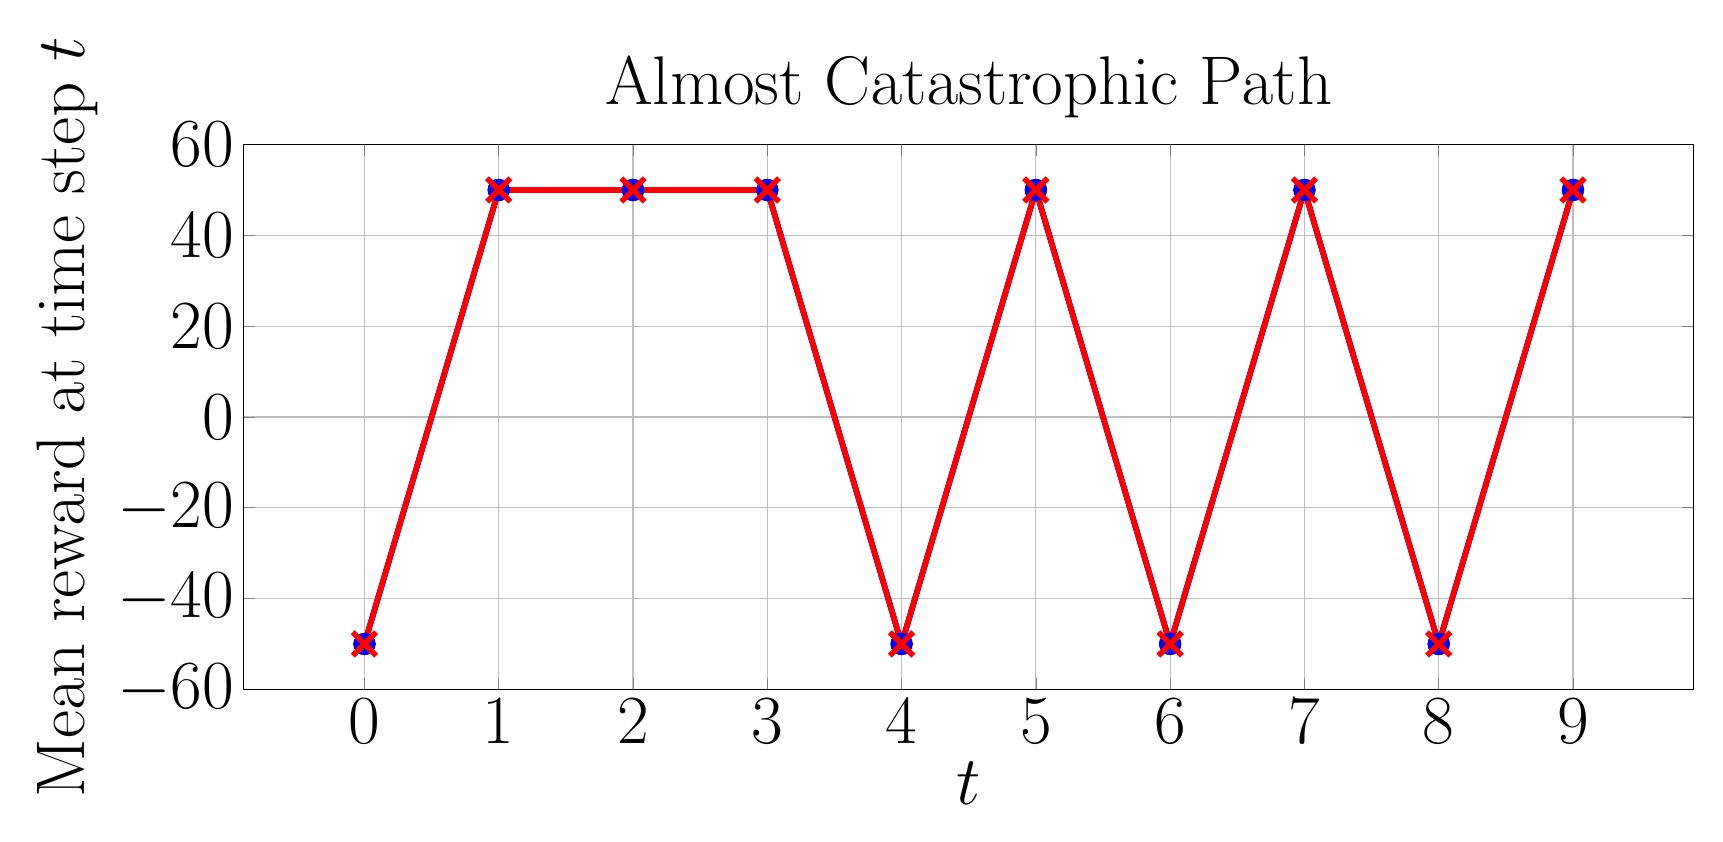
\begin{tikzpicture}
                \begin{axis}[
                    xlabel={$t$},
                    ylabel={Mean reward at time step $t$},
                    title={Almost Catastrophic Path},
                    grid=both,
                    every axis/.style={font=\Huge},
                    width=20cm, height=8.5cm,
                    %
                ]
               \addplot[
                    color=black, %
                    mark=*, %
                    line width=2pt,
                    mark size=3pt,
                ]
                coordinates {
                    (0, -50.0)
                    (1, 50.0)
                    (2, 50.0)
                    (3, 50.0)
                    (4, -50.0)
                    (5, 50.0)
                    (6, -50.0)
                    (7, 50.0)
                    (8, -50.0)
                    (9, 50.0)
                };
                %
                %
                \addplot[
                    color=blue, %
                    mark=o, %
                    line width=2pt,
                    mark size=3pt,
                    error bars/.cd,
                    y dir=both, %
                    y explicit, %
                    error bar style={line width=1pt,solid},
                    error mark options={line width=1pt,mark size=4pt,rotate=90}
                ]
                coordinates {
                    (0, -50.0)  +- (0, 0.0)
                    (1, 50.0)  +- (0, 0.0) 
                    (2, 50.0)  +- (0, 0.0) 
                    (3, 50.0)  +- (0, 0.0)
                    (4, -50.0)  +- (0, 0.0)
                    (5, 50.0) +- (0, 0.0)
                    (6, -50.0) +- (0, 0.0)
                    (7, 50.0) +- (0, 0.0)
                    (8, -50.0) +- (0, 0.0)
                    (9, 50.0) +- (0, 0.0)
                };
                %
                \addplot[
                    color=red, %
                    mark=x, %
                    line width=2pt,
                    mark size=6pt,
                    error bars/.cd,
                    y dir=both, %
                    y explicit, %
                    error bar style={line width=1pt,solid},
                    error mark options={line width=1pt,mark size=4pt,rotate=90}
                ]
                coordinates {
                    (0, -50.0)  +- (0, 0.0)
                    (1, 50.0)  +- (0, 0.0) 
                    (2, 50.0)  +- (0, 0.0) 
                    (3, 50.0)  +- (0, 0.0)
                    (4, -50.0)  +- (0, 0.0)
                    (5, 50.0) +- (0, 0.0)
                    (6, -50.0) +- (0, 0.0)
                    (7, 50.0) +- (0, 0.0)
                    (8, -50.0) +- (0, 0.0)
                    (9, 50.0) +- (0, 0.0)
                };
                %
                %
                %
                %
                %
                %
                %
                %
                %
                %
                %
                %
                %
                %
                %
                %
                %
                %
                %
                \end{axis}
            \end{tikzpicture}
         }
    }
    \hspace{1cm}
    \subfigure[\footnotesize Lowest cumulative reward: Interval CFMDP ($-7150$), Gumbel-max SCM ($-9050$)]{%
         \resizebox{0.76\columnwidth}{!}{
            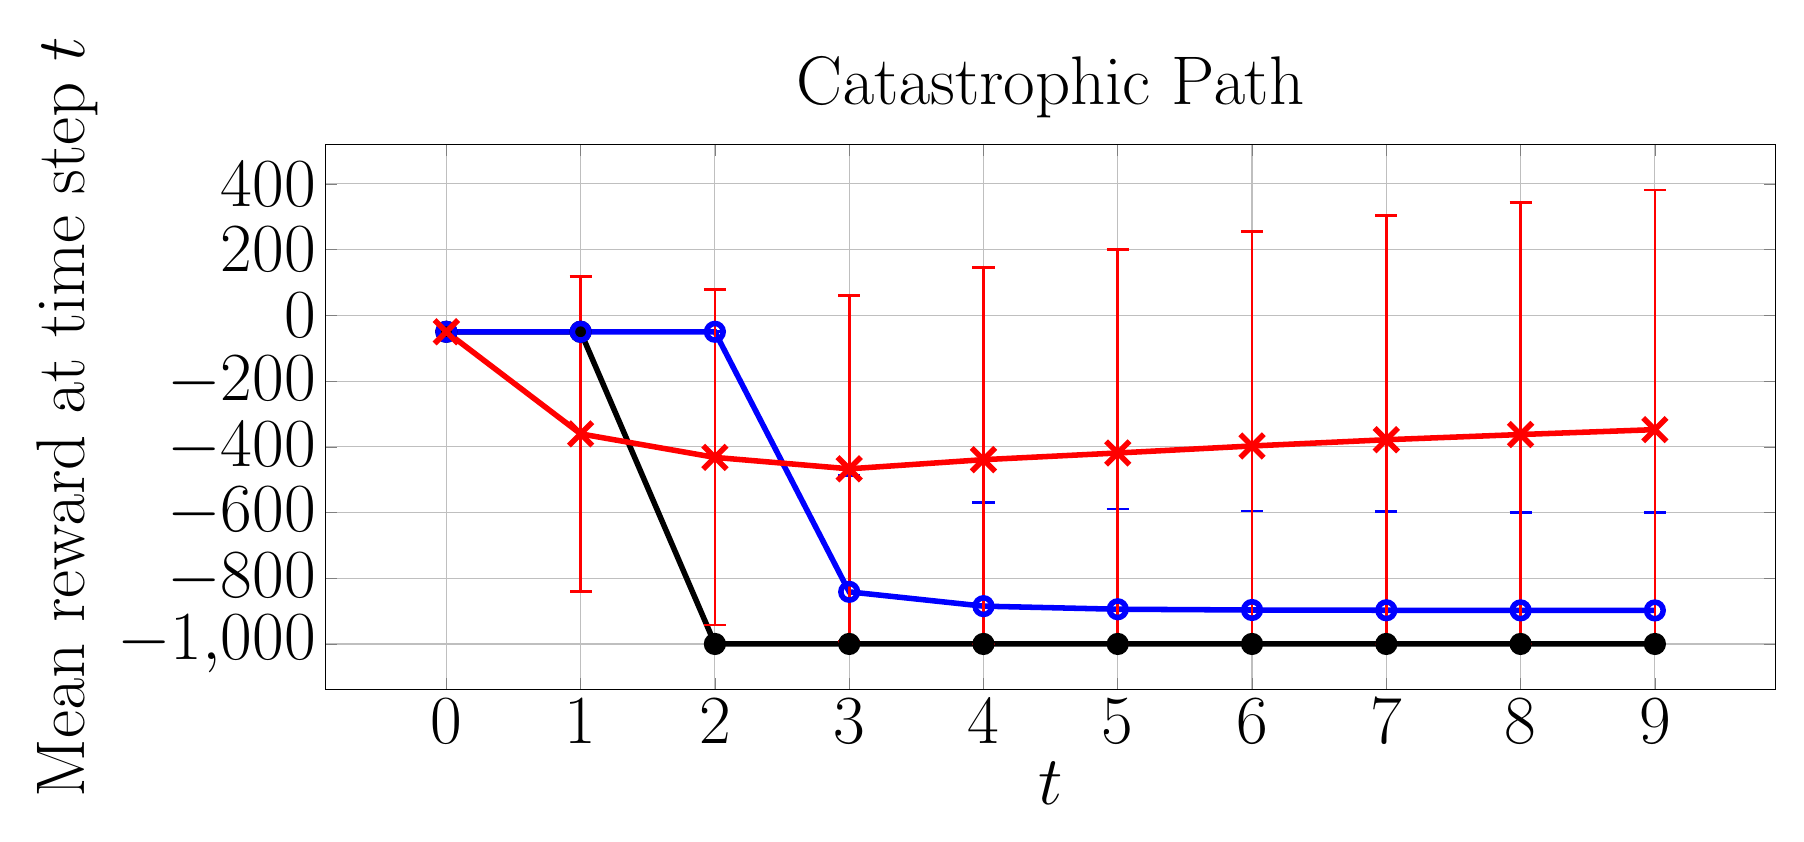
\begin{tikzpicture}
                \begin{axis}[
                    xlabel={$t$},
                    ylabel={Mean reward at time step $t$},
                    title={Catastrophic Path},
                    grid=both,
                    width=20cm, height=8.5cm,
                    every axis/.style={font=\Huge},
                    %
                ]
               \addplot[
                    color=black, %
                    mark=*, %
                    line width=2pt,
                    mark size=3pt,
                ]
                coordinates {
                    (0, -50.0)
                    (1, -50.0)
                    (2, -1000.0)
                    (3, -1000.0)
                    (4, -1000.0)
                    (5, -1000.0)
                    (6, -1000.0)
                    (7, -1000.0)
                    (8, -1000.0)
                    (9, -1000.0)
                };
                %
                %
                \addplot[
                    color=blue, %
                    mark=o, %
                    line width=2pt,
                    mark size=3pt,
                    error bars/.cd,
                    y dir=both, %
                    y explicit, %
                    error bar style={line width=1pt,solid},
                    error mark options={line width=1pt,mark size=4pt,rotate=90}
                ]
                coordinates {
                    (0, -50.0)  +- (0, 0.0)
                    (1, -50.0)  +- (0, 0.0) 
                    (2, -50.0)  +- (0, 0.0) 
                    (3, -841.440725)  += (0, 354.24605512) -= (0, 158.559275)
                    (4, -884.98225)  += (0, 315.37519669) -= (0, 115.01775)
                    (5, -894.330425) += (0, 304.88572805) -= (0, 105.669575)
                    (6, -896.696175) += (0, 301.19954514) -= (0, 103.303825)
                    (7, -897.4635) += (0, 299.61791279) -= (0, 102.5365)
                    (8, -897.77595) += (0, 298.80392585) -= (0, 102.22405)
                    (9, -897.942975) += (0, 298.32920557) -= (0, 102.057025)
                };
                %
                \addplot[
                    color=red, %
                    mark=x, %
                    line width=2pt,
                    mark size=6pt,
                    error bars/.cd,
                    y dir=both, %
                    y explicit, %
                    error bar style={line width=1pt,solid},
                    error mark options={line width=1pt,mark size=4pt,rotate=90}
                ]
            coordinates {
                    (0, -50.0)  +- (0, 0.0)
                    (1, -360.675265)  +- (0, 479.39812699) 
                    (2, -432.27629)  +- (0, 510.38620897) 
                    (3, -467.029545)  += (0, 526.36009628) -= (0, 526.36009628)
                    (4, -439.17429)  += (0, 583.96638919) -= (0, 560.82571)
                    (5, -418.82704) += (0, 618.43027478) -= (0, 581.17296)
                    (6, -397.464895) += (0, 652.67322574) -= (0, 602.535105)
                    (7, -378.49052) += (0, 682.85407033) -= (0, 621.50948)
                    (8, -362.654195) += (0, 707.01412023) -= (0, 637.345805)
                    (9, -347.737935) += (0, 729.29076479) -= (0, 652.262065)
                };
                %
                %
                %
                %
                %
                %
                %
                %
                %
                %
                %
                %
                %
                %
                %
                %
                %
                %
                %
                \end{axis}
            \end{tikzpicture}
         }
    }
    \caption{Average instant reward of CF paths induced by policies on Sepsis.}
    \label{fig: reward sepsis}
\end{figure*}

%
%
%
\subsection{Interval CFMDP Bounds}
%
%
Table \ref{tab:nonzero_probs} presents the mean counterfactual probability bound widths (excluding transitions where the upper bound is $0$) for each MDP, averaged over 20 observed paths. We compare the bounds under counterfactual stability (CS) and monotonicity (M) assumptions, CS alone, and no assumptions. This shows that the assumptions marginally reduce the bound widths, indicating the assumptions tighten the bounds without excluding too many causal models, as intended.
\renewcommand{\arraystretch}{1}

\begin{table}
\centering
\caption{Mean width of counterfactual probability bounds}
\resizebox{0.8\columnwidth}{!}{%
\begin{tabular}{|c|c|c|c|}
\hline
\multirow{2}{*}{\textbf{Environment}} & \multicolumn{3}{c|}{\textbf{Assumptions}} \\ \cline{2-4}
 & \textbf{CS + M} & \textbf{CS} & \textbf{None\tablefootnote{\jl{Equivalent to \citet{li2024probabilities}'s bounds (see Section \ref{sec: equivalence with Li}).}}} \\ \hline
\textbf{GridWorld} ($p=0.9$) & 0.0817 & 0.0977 & 0.100 \\ \hline
\textbf{GridWorld} ($p=0.4$) & 0.552  & 0.638  & 0.646 \\ \hline
\textbf{Sepsis} & 0.138 & 0.140 & 0.140 \\ \hline
\end{tabular}
}
\label{tab:nonzero_probs}
\end{table}


\subsection{Execution Times}
Table \ref{tab: times} compares the average time needed to generate the interval CFMDP vs.\ the Gumbel-max SCM CFMDP for 20 observations.
The GridWorld algorithms were run single-threaded, while the Sepsis experiments were run in parallel.
Generating the interval CFMDP is significantly faster as it uses exact analytical bounds, whereas the Gumbel-max CFMDP requires sampling from the Gumbel distribution to estimate counterfactual transition probabilities. \jl{Since constructing the counterfactual MDP models is the main bottleneck in both approaches, ours is more efficient overall and suitable for larger MDPs.}
\begin{table}
\centering
\caption{Mean execution time to generate CFMDPs}
\resizebox{0.99\columnwidth}{!}{%
\begin{tabular}{|c|c|c|}
\hline
\multirow{2}{*}{\textbf{Environment}} & \multicolumn{2}{c|}{\textbf{Mean Execution Time (s)}} \\ \cline{2-3} 
                                      & \textbf{Interval CFMDP} & \textbf{Gumbel-max CFMDP} \\ \hline
\textbf{GridWorld ($p=0.9$) }                  & 0.261                   & 56.1                      \\ \hline
\textbf{GridWorld ($p=0.4$)  }                 & 0.336                   & 54.5                      \\ \hline
\textbf{Sepsis}                                 & 688                     & 2940                      \\ \hline
\end{tabular}%
}
\label{tab: times}
\end{table}

% \ifpdf
\DeclareGraphicsExtensions{.eps,.pdf,.png,.jpg}
\else
\DeclareGraphicsExtensions{.eps}
\fi

% Prevent itemized lists from running into the left margin inside theorems and proofs
\setlist[enumerate]{leftmargin=.5in}
\setlist[itemize]{leftmargin=.5in}

% Add a serial/Oxford comma by default.
\newcommand{\creflastconjunction}{, and~}

% Setting for algorithms
\Crefname{ALC@unique}{Line}{Lines}

% Tikz libraries
\usetikzlibrary{positioning}
\usetikzlibrary{calc}
\usetikzlibrary{shapes.geometric}
\usetikzlibrary{angles}
\usetikzlibrary{decorations.pathreplacing}
\usetikzlibrary{calligraphy}

% 
\begin{table*}[t]
\centering
\fontsize{11pt}{11pt}\selectfont
\begin{tabular}{lllllllllllll}
\toprule
\multicolumn{1}{c}{\textbf{task}} & \multicolumn{2}{c}{\textbf{Mir}} & \multicolumn{2}{c}{\textbf{Lai}} & \multicolumn{2}{c}{\textbf{Ziegen.}} & \multicolumn{2}{c}{\textbf{Cao}} & \multicolumn{2}{c}{\textbf{Alva-Man.}} & \multicolumn{1}{c}{\textbf{avg.}} & \textbf{\begin{tabular}[c]{@{}l@{}}avg.\\ rank\end{tabular}} \\
\multicolumn{1}{c}{\textbf{metrics}} & \multicolumn{1}{c}{\textbf{cor.}} & \multicolumn{1}{c}{\textbf{p-v.}} & \multicolumn{1}{c}{\textbf{cor.}} & \multicolumn{1}{c}{\textbf{p-v.}} & \multicolumn{1}{c}{\textbf{cor.}} & \multicolumn{1}{c}{\textbf{p-v.}} & \multicolumn{1}{c}{\textbf{cor.}} & \multicolumn{1}{c}{\textbf{p-v.}} & \multicolumn{1}{c}{\textbf{cor.}} & \multicolumn{1}{c}{\textbf{p-v.}} &  &  \\ \midrule
\textbf{S-Bleu} & 0.50 & 0.0 & 0.47 & 0.0 & 0.59 & 0.0 & 0.58 & 0.0 & 0.68 & 0.0 & 0.57 & 5.8 \\
\textbf{R-Bleu} & -- & -- & 0.27 & 0.0 & 0.30 & 0.0 & -- & -- & -- & -- & - &  \\
\textbf{S-Meteor} & 0.49 & 0.0 & 0.48 & 0.0 & 0.61 & 0.0 & 0.57 & 0.0 & 0.64 & 0.0 & 0.56 & 6.1 \\
\textbf{R-Meteor} & -- & -- & 0.34 & 0.0 & 0.26 & 0.0 & -- & -- & -- & -- & - &  \\
\textbf{S-Bertscore} & \textbf{0.53} & 0.0 & {\ul 0.80} & 0.0 & \textbf{0.70} & 0.0 & {\ul 0.66} & 0.0 & {\ul0.78} & 0.0 & \textbf{0.69} & \textbf{1.7} \\
\textbf{R-Bertscore} & -- & -- & 0.51 & 0.0 & 0.38 & 0.0 & -- & -- & -- & -- & - &  \\
\textbf{S-Bleurt} & {\ul 0.52} & 0.0 & {\ul 0.80} & 0.0 & 0.60 & 0.0 & \textbf{0.70} & 0.0 & \textbf{0.80} & 0.0 & {\ul 0.68} & {\ul 2.3} \\
\textbf{R-Bleurt} & -- & -- & 0.59 & 0.0 & -0.05 & 0.13 & -- & -- & -- & -- & - &  \\
\textbf{S-Cosine} & 0.51 & 0.0 & 0.69 & 0.0 & {\ul 0.62} & 0.0 & 0.61 & 0.0 & 0.65 & 0.0 & 0.62 & 4.4 \\
\textbf{R-Cosine} & -- & -- & 0.40 & 0.0 & 0.29 & 0.0 & -- & -- & -- & -- & - & \\ \midrule
\textbf{QuestEval} & 0.23 & 0.0 & 0.25 & 0.0 & 0.49 & 0.0 & 0.47 & 0.0 & 0.62 & 0.0 & 0.41 & 9.0 \\
\textbf{LLaMa3} & 0.36 & 0.0 & \textbf{0.84} & 0.0 & {\ul{0.62}} & 0.0 & 0.61 & 0.0 &  0.76 & 0.0 & 0.64 & 3.6 \\
\textbf{our (3b)} & 0.49 & 0.0 & 0.73 & 0.0 & 0.54 & 0.0 & 0.53 & 0.0 & 0.7 & 0.0 & 0.60 & 5.8 \\
\textbf{our (8b)} & 0.48 & 0.0 & 0.73 & 0.0 & 0.52 & 0.0 & 0.53 & 0.0 & 0.7 & 0.0 & 0.59 & 6.3 \\  \bottomrule
\end{tabular}
\caption{Pearson correlation on human evaluation on system output. `R-': reference-based. `S-': source-based.}
\label{tab:sys}
\end{table*}



\begin{table}%[]
\centering
\fontsize{11pt}{11pt}\selectfont
\begin{tabular}{llllll}
\toprule
\multicolumn{1}{c}{\textbf{task}} & \multicolumn{1}{c}{\textbf{Lai}} & \multicolumn{1}{c}{\textbf{Zei.}} & \multicolumn{1}{c}{\textbf{Scia.}} & \textbf{} & \textbf{} \\ 
\multicolumn{1}{c}{\textbf{metrics}} & \multicolumn{1}{c}{\textbf{cor.}} & \multicolumn{1}{c}{\textbf{cor.}} & \multicolumn{1}{c}{\textbf{cor.}} & \textbf{avg.} & \textbf{\begin{tabular}[c]{@{}l@{}}avg.\\ rank\end{tabular}} \\ \midrule
\textbf{S-Bleu} & 0.40 & 0.40 & 0.19* & 0.33 & 7.67 \\
\textbf{S-Meteor} & 0.41 & 0.42 & 0.16* & 0.33 & 7.33 \\
\textbf{S-BertS.} & {\ul0.58} & 0.47 & 0.31 & 0.45 & 3.67 \\
\textbf{S-Bleurt} & 0.45 & {\ul 0.54} & {\ul 0.37} & 0.45 & {\ul 3.33} \\
\textbf{S-Cosine} & 0.56 & 0.52 & 0.3 & {\ul 0.46} & {\ul 3.33} \\ \midrule
\textbf{QuestE.} & 0.27 & 0.35 & 0.06* & 0.23 & 9.00 \\
\textbf{LlaMA3} & \textbf{0.6} & \textbf{0.67} & \textbf{0.51} & \textbf{0.59} & \textbf{1.0} \\
\textbf{Our (3b)} & 0.51 & 0.49 & 0.23* & 0.39 & 4.83 \\
\textbf{Our (8b)} & 0.52 & 0.49 & 0.22* & 0.43 & 4.83 \\ \bottomrule
\end{tabular}
\caption{Pearson correlation on human ratings on reference output. *not significant; we cannot reject the null hypothesis of zero correlation}
\label{tab:ref}
\end{table}


\begin{table*}%[]
\centering
\fontsize{11pt}{11pt}\selectfont
\begin{tabular}{lllllllll}
\toprule
\textbf{task} & \multicolumn{1}{c}{\textbf{ALL}} & \multicolumn{1}{c}{\textbf{sentiment}} & \multicolumn{1}{c}{\textbf{detoxify}} & \multicolumn{1}{c}{\textbf{catchy}} & \multicolumn{1}{c}{\textbf{polite}} & \multicolumn{1}{c}{\textbf{persuasive}} & \multicolumn{1}{c}{\textbf{formal}} & \textbf{\begin{tabular}[c]{@{}l@{}}avg. \\ rank\end{tabular}} \\
\textbf{metrics} & \multicolumn{1}{c}{\textbf{cor.}} & \multicolumn{1}{c}{\textbf{cor.}} & \multicolumn{1}{c}{\textbf{cor.}} & \multicolumn{1}{c}{\textbf{cor.}} & \multicolumn{1}{c}{\textbf{cor.}} & \multicolumn{1}{c}{\textbf{cor.}} & \multicolumn{1}{c}{\textbf{cor.}} &  \\ \midrule
\textbf{S-Bleu} & -0.17 & -0.82 & -0.45 & -0.12* & -0.1* & -0.05 & -0.21 & 8.42 \\
\textbf{R-Bleu} & - & -0.5 & -0.45 &  &  &  &  &  \\
\textbf{S-Meteor} & -0.07* & -0.55 & -0.4 & -0.01* & 0.1* & -0.16 & -0.04* & 7.67 \\
\textbf{R-Meteor} & - & -0.17* & -0.39 & - & - & - & - & - \\
\textbf{S-BertScore} & 0.11 & -0.38 & -0.07* & -0.17* & 0.28 & 0.12 & 0.25 & 6.0 \\
\textbf{R-BertScore} & - & -0.02* & -0.21* & - & - & - & - & - \\
\textbf{S-Bleurt} & 0.29 & 0.05* & 0.45 & 0.06* & 0.29 & 0.23 & 0.46 & 4.2 \\
\textbf{R-Bleurt} & - &  0.21 & 0.38 & - & - & - & - & - \\
\textbf{S-Cosine} & 0.01* & -0.5 & -0.13* & -0.19* & 0.05* & -0.05* & 0.15* & 7.42 \\
\textbf{R-Cosine} & - & -0.11* & -0.16* & - & - & - & - & - \\ \midrule
\textbf{QuestEval} & 0.21 & {\ul{0.29}} & 0.23 & 0.37 & 0.19* & 0.35 & 0.14* & 4.67 \\
\textbf{LlaMA3} & \textbf{0.82} & \textbf{0.80} & \textbf{0.72} & \textbf{0.84} & \textbf{0.84} & \textbf{0.90} & \textbf{0.88} & \textbf{1.00} \\
\textbf{Our (3b)} & 0.47 & -0.11* & 0.37 & 0.61 & 0.53 & 0.54 & 0.66 & 3.5 \\
\textbf{Our (8b)} & {\ul{0.57}} & 0.09* & {\ul 0.49} & {\ul 0.72} & {\ul 0.64} & {\ul 0.62} & {\ul 0.67} & {\ul 2.17} \\ \bottomrule
\end{tabular}
\caption{Pearson correlation on human ratings on our constructed test set. 'R-': reference-based. 'S-': source-based. *not significant; we cannot reject the null hypothesis of zero correlation}
\label{tab:con}
\end{table*}

\section{Results}
We benchmark the different metrics on the different datasets using correlation to human judgement. For content preservation, we show results split on data with system output, reference output and our constructed test set: we show that the data source for evaluation leads to different conclusions on the metrics. In addition, we examine whether the metrics can rank style transfer systems similar to humans. On style strength, we likewise show correlations between human judgment and zero-shot evaluation approaches. When applicable, we summarize results by reporting the average correlation. And the average ranking of the metric per dataset (by ranking which metric obtains the highest correlation to human judgement per dataset). 

\subsection{Content preservation}
\paragraph{How do data sources affect the conclusion on best metric?}
The conclusions about the metrics' performance change radically depending on whether we use system output data, reference output, or our constructed test set. Ideally, a good metric correlates highly with humans on any data source. Ideally, for meta-evaluation, a metric should correlate consistently across all data sources, but the following shows that the correlations indicate different things, and the conclusion on the best metric should be drawn carefully.

Looking at the metrics correlations with humans on the data source with system output (Table~\ref{tab:sys}), we see a relatively high correlation for many of the metrics on many tasks. The overall best metrics are S-BertScore and S-BLEURT (avg+avg rank). We see no notable difference in our method of using the 3B or 8B model as the backbone.

Examining the average correlations based on data with reference output (Table~\ref{tab:ref}), now the zero-shoot prompting with LlaMA3 70B is the best-performing approach ($0.59$ avg). Tied for second place are source-based cosine embedding ($0.46$ avg), BLEURT ($0.45$ avg) and BertScore ($0.45$ avg). Our method follows on a 5. place: here, the 8b version (($0.43$ avg)) shows a bit stronger results than 3b ($0.39$ avg). The fact that the conclusions change, whether looking at reference or system output, confirms the observations made by \citet{scialom-etal-2021-questeval} on simplicity transfer.   

Now consider the results on our test set (Table~\ref{tab:con}): Several metrics show low or no correlation; we even see a significantly negative correlation for some metrics on ALL (BLEU) and for specific subparts of our test set for BLEU, Meteor, BertScore, Cosine. On the other end, LlaMA3 70B is again performing best, showing strong results ($0.82$ in ALL). The runner-up is now our 8B method, with a gap to the 3B version ($0.57$ vs $0.47$ in ALL). Note our method still shows zero correlation for the sentiment task. After, ranks BLEURT ($0.29$), QuestEval ($0.21$), BertScore ($0.11$), Cosine ($0.01$).  

On our test set, we find that some metrics that correlate relatively well on the other datasets, now exhibit low correlation. Hence, with our test set, we can now support the logical reasoning with data evidence: Evaluation of content preservation for style transfer needs to take the style shift into account. This conclusion could not be drawn using the existing data sources: We hypothesise that for the data with system-based output, successful output happens to be very similar to the source sentence and vice versa, and reference-based output might not contain server mistakes as they are gold references. Thus, none of the existing data sources tests the limits of the metrics.  


\paragraph{How do reference-based metrics compare to source-based ones?} Reference-based metrics show a lower correlation than the source-based counterpart for all metrics on both datasets with ratings on references (Table~\ref{tab:sys}). As discussed previously, reference-based metrics for style transfer have the drawback that many different good solutions on a rewrite might exist and not only one similar to a reference.


\paragraph{How well can the metrics rank the performance of style transfer methods?}
We compare the metrics' ability to judge the best style transfer methods w.r.t. the human annotations: Several of the data sources contain samples from different style transfer systems. In order to use metrics to assess the quality of the style transfer system, metrics should correctly find the best-performing system. Hence, we evaluate whether the metrics for content preservation provide the same system ranking as human evaluators. We take the mean of the score for every output on each system and the mean of the human annotations; we compare the systems using the Kendall's Tau correlation. 

We find only the evaluation using the dataset Mir, Lai, and Ziegen to result in significant correlations, probably because of sparsity in a number of system tests (App.~\ref{app:dataset}). Our method (8b) is the only metric providing a perfect ranking of the style transfer system on the Lai data, and Llama3 70B the only one on the Ziegen data. Results in App.~\ref{app:results}. 


\subsection{Style strength results}
%Evaluating style strengths is a challenging task. 
Llama3 70B shows better overall results than our method. However, our method scores higher than Llama3 70B on 2 out of 6 datasets, but it also exhibits zero correlation on one task (Table~\ref{tab:styleresults}).%More work i s needed on evaluating style strengths. 
 
\begin{table}%[]
\fontsize{11pt}{11pt}\selectfont
\begin{tabular}{lccc}
\toprule
\multicolumn{1}{c}{\textbf{}} & \textbf{LlaMA3} & \textbf{Our (3b)} & \textbf{Our (8b)} \\ \midrule
\textbf{Mir} & 0.46 & 0.54 & \textbf{0.57} \\
\textbf{Lai} & \textbf{0.57} & 0.18 & 0.19 \\
\textbf{Ziegen.} & 0.25 & 0.27 & \textbf{0.32} \\
\textbf{Alva-M.} & \textbf{0.59} & 0.03* & 0.02* \\
\textbf{Scialom} & \textbf{0.62} & 0.45 & 0.44 \\
\textbf{\begin{tabular}[c]{@{}l@{}}Our Test\end{tabular}} & \textbf{0.63} & 0.46 & 0.48 \\ \bottomrule
\end{tabular}
\caption{Style strength: Pearson correlation to human ratings. *not significant; we cannot reject the null hypothesis of zero corelation}
\label{tab:styleresults}
\end{table}

\subsection{Ablation}
We conduct several runs of the methods using LLMs with variations in instructions/prompts (App.~\ref{app:method}). We observe that the lower the correlation on a task, the higher the variation between the different runs. For our method, we only observe low variance between the runs.
None of the variations leads to different conclusions of the meta-evaluation. Results in App.~\ref{app:results}.
% \begin{table}[!t]
% \centering
% \scalebox{0.68}{
%     \begin{tabular}{ll cccc}
%       \toprule
%       & \multicolumn{4}{c}{\textbf{Intellipro Dataset}}\\
%       & \multicolumn{2}{c}{Rank Resume} & \multicolumn{2}{c}{Rank Job} \\
%       \cmidrule(lr){2-3} \cmidrule(lr){4-5} 
%       \textbf{Method}
%       &  Recall@100 & nDCG@100 & Recall@10 & nDCG@10 \\
%       \midrule
%       \confitold{}
%       & 71.28 &34.79 &76.50 &52.57 
%       \\
%       \cmidrule{2-5}
%       \confitsimple{}
%     & 82.53 &48.17
%        & 85.58 &64.91
     
%        \\
%        +\RunnerUpMiningShort{}
%     &85.43 &50.99 &91.38 &71.34 
%       \\
%       +\HyReShort
%         &- & -
%        &-&-\\
       
%       \bottomrule

%     \end{tabular}
%   }
% \caption{Ablation studies using Jina-v2-base as the encoder. ``\confitsimple{}'' refers using a simplified encoder architecture. \framework{} trains \confitsimple{} with \RunnerUpMiningShort{} and \HyReShort{}.}
% \label{tbl:ablation}
% \end{table}
\begin{table*}[!t]
\centering
\scalebox{0.75}{
    \begin{tabular}{l cccc cccc}
      \toprule
      & \multicolumn{4}{c}{\textbf{Recruiting Dataset}}
      & \multicolumn{4}{c}{\textbf{AliYun Dataset}}\\
      & \multicolumn{2}{c}{Rank Resume} & \multicolumn{2}{c}{Rank Job} 
      & \multicolumn{2}{c}{Rank Resume} & \multicolumn{2}{c}{Rank Job}\\
      \cmidrule(lr){2-3} \cmidrule(lr){4-5} 
      \cmidrule(lr){6-7} \cmidrule(lr){8-9} 
      \textbf{Method}
      & Recall@100 & nDCG@100 & Recall@10 & nDCG@10
      & Recall@100 & nDCG@100 & Recall@10 & nDCG@10\\
      \midrule
      \confitold{}
      & 71.28 & 34.79 & 76.50 & 52.57 
      & 87.81 & 65.06 & 72.39 & 56.12
      \\
      \cmidrule{2-9}
      \confitsimple{}
      & 82.53 & 48.17 & 85.58 & 64.91
      & 94.90&78.40 & 78.70& 65.45
       \\
      +\HyReShort{}
       &85.28 & 49.50
       &90.25 & 70.22
       & 96.62&81.99 & \textbf{81.16}& 67.63
       \\
      +\RunnerUpMiningShort{}
       % & 85.14& 49.82
       % &90.75&72.51
       & \textbf{86.13}&\textbf{51.90} & \textbf{94.25}&\textbf{73.32}
       & \textbf{97.07}&\textbf{83.11} & 80.49& \textbf{68.02}
       \\
   %     +\RunnerUpMiningShort{}
   %    & 85.43 & 50.99 & 91.38 & 71.34 
   %    & 96.24 & 82.95 & 80.12 & 66.96
   %    \\
   %    +\HyReShort{} old
   %     &85.28 & 49.50
   %     &90.25 & 70.22
   %     & 96.62&81.99 & 81.16& 67.63
   %     \\
   % +\HyReShort{} 
   %     % & 85.14& 49.82
   %     % &90.75&72.51
   %     & 86.83&51.77 &92.00 &72.04
   %     & 97.07&83.11 & 80.49& 68.02
   %     \\
      \bottomrule

    \end{tabular}
  }
\caption{\framework{} ablation studies. ``\confitsimple{}'' refers using a simplified encoder architecture. \framework{} trains \confitsimple{} with \RunnerUpMiningShort{} and \HyReShort{}. We use Jina-v2-base as the encoder due to its better performance.
}
\label{tbl:ablation}
\end{table*}
\section{Conclusion}
In this work, we propose a simple yet effective approach, called SMILE, for graph few-shot learning with fewer tasks. Specifically, we introduce a novel dual-level mixup strategy, including within-task and across-task mixup, for enriching the diversity of nodes within each task and the diversity of tasks. Also, we incorporate the degree-based prior information to learn expressive node embeddings. Theoretically, we prove that SMILE effectively enhances the model's generalization performance. Empirically, we conduct extensive experiments on multiple benchmarks and the results suggest that SMILE significantly outperforms other baselines, including both in-domain and cross-domain few-shot settings.

% %-------------------------------------------------------------------------------
% \section*{Availability}
%-------------------------------------------------------------------------------

% %-------------------------------------------------------------------------------
\section*{Ethics Considerations}
% %-------------------------------------------------------------------------------
In this work, we propose a novel adversarial machine learning attack and conduct experiments exclusively in controlled, lab-only environments. Our primary goal is to advance the understanding of adversarial vulnerabilities in machine learning systems and to contribute to the development of more robust defenses. All experiments were carried out with benchmark datasets or models designed for research purposes, ensuring no real-world harm or exploitation of sensitive data. We acknowledge the dual-use nature of adversarial research and emphasize our commitment to ethical guidelines by openly discussing mitigation strategies and encouraging responsible use of this work.
%-------------------------------------------------------------------------------
\section*{Open Science}
% %-------------------------------------------------------------------------------

All the resources required for reproducing the experiments described in this study are provided.
This includes the complete dataset (traditional benchmarks), pre-processing scripts, model training code, and detailed instructions for setting up the computational environment. By ensuring accessibility to these resources, we aim to facilitate transparency, reproducibility, and further research in the field of ML.
All supplementary materials are available in the accompanying repository, providing a comprehensive framework for replicating and validating our findings.
% GitHub repository: \url{https://anonymous.4open.science/r/MOSHI-1518}.

\balance
\bibliographystyle{plain}
\bibliography{bibliography}

% \appendix
% \section{Data Availability}
% All the resources required for reproducing the experiments described in this study are provided. This includes the complete dataset (traditional benchmarks), pre-processing scripts, and model training code, as well as detailed instructions for setting up the computational environment. By ensuring accessibility to these resources, we aim to facilitate transparency, reproducibility, and further research in the field of machine learning. All supplementary materials are available in the accompanying repository, providing a comprehensive framework for replication and validation of our findings. GitHub repository: 
% \url{https://anonymous.4open.science/r/MSHAA-68DD/README.md}

%%%%%%%%%%%%%%%%%%%%%%%%%%%%%%%%%%%%%%%%%%%%%%%%%%%%%%%%%%%%%%%%%%%%%%%%%%%%%%%%
\end{document}
%%%%%%%%%%%%%%%%%%%%%%%%%%%%%%%%%%%%%%%%%%%%%%%%%%%%%%%%%%%%%%%%%%%%%%%%%%%%%%%%

%%  LocalWords:  endnotes includegraphics fread ptr nobj noindent
%%  LocalWords:  pdflatex acks